% =====================================================================
% Multi-ViT Feature Fusion for HyperKvasir 23-class Classification
% Final report — complete draft (Overleaf / pdfLaTeX compatible).
% Report language: Turkish (assignment §5; academic register).
%
% Report checks:
%   - Every number traces to saved outputs or cited sources; no invention.
%   - macro-F1 is the primary metric; accuracy is supporting only.
%   - Literature comparisons that use a different protocol are CONTEXTUAL only.
%   - No best-in-literature claims. Classifier is MLP only.
% =====================================================================
\documentclass[11pt,a4paper]{article}

% Encoding and language
% Cross-engine: pdfLaTeX/Overleaf uses inputenc+fontenc (the target toolchain);
% XeLaTeX/LuaLaTeX (e.g. local `tectonic`) uses fontspec for native Unicode so
% Turkish glyphs (ı, ş, ğ, ç, ö, ü) render correctly under either engine.
\usepackage{iftex}
\ifPDFTeX
  \usepackage[utf8]{inputenc}
  \usepackage[T1]{fontenc}
  \usepackage{lmodern}
\else
  \usepackage{fontspec}
\fi
\usepackage[turkish]{babel}
% Turkish babel makes '=' an active shorthand, which breaks '=' inside
% \includegraphics[width=...], TikZ option lists, etc. Disable it globally
% (it only controls explicit hyphenation hints; normal text is unaffected).
\AtBeginDocument{\shorthandoff{=}}

% Packages
\usepackage[margin=2.5cm]{geometry}
\usepackage{amsmath}
\usepackage{amssymb}
\usepackage{graphicx}
\usepackage{booktabs}
\usepackage{tabularx}
\usepackage{float}
\usepackage{caption}
\usepackage{subcaption}
\usepackage{xcolor}
\usepackage{tikz}
\usetikzlibrary{positioning, arrows.meta}
\usepackage{hyperref}

\graphicspath{{figures/}}

\hypersetup{
  colorlinks=true,
  linkcolor=black,
  citecolor=black,
  urlcolor=blue
}

% =====================================================================
\title{Çoklu ViT Tabanlı Özellik Füzyonu ile HiperKvasir\\
       23-Sınıf Gastrointestinal Görüntü Sınıflandırması}
\author{Yasin Ekici \\ Öğrenci No: 21360859029 \\[4pt]
  \small \url{https://github.com/YasinEkici/hyperkvasir-multi-backbone-fusion}}
\date{\today}

\begin{document}

\maketitle

\begin{abstract}
Bu çalışmada, HiperKvasir veri kümesindeki 23 sınıflı ve sınıf dağılımı oldukça
dengesiz gastrointestinal endoskopi görüntü sınıflandırması problemi ele
alınmaktadır. Önceden eğitilmiş üç görüntü dönüştürücü (Vision Transformer)
omurga ağı (ViT-B/16, Swin-T ve BEiT-B/16) özellik çıkarıcı olarak
kullanılmış; her daldan elde edilen 768 boyutlu havuzlanmış öznitelikler 512
boyuta izdüşürülerek birleştirme (concatenation), ağırlıklı ve gelişmiş bir
kapılı (GMU) füzyon yöntemiyle birleştirilmiş ve sabit bir çok katmanlı
algılayıcı (MLP) ile sınıflandırılmıştır. Hem dondurulmuş öznitelik çıkarımı hem
de son dönüştürücü bloklarının ince ayarı (fine-tune) değerlendirilmiştir.
Değerlendirme, sızıntıya karşı denetlenmiş resmi 5-katlı protokol altında
yürütülmüş; ana ölçüt olarak makro-F1, destekleyici ölçüt olarak doğruluk
kullanılmış ve sonuçlar önyükleme (bootstrap) \%95 güven aralıklarıyla
raporlanmıştır. Çapraz doğrulamada en iyi yapılandırma, üç omurganın ağırlıklı
füzyonunun ince ayarlı sürümü olmuştur (havuzlanmış makro-F1 $0{,}6119$, \%95 GA
$[0{,}5930,\,0{,}6295]$; doğruluk $\approx 0{,}88$). Bu yapılandırma, eşli
McNemar testinde en iyi tekli omurgadan ve en iyi ikili füzyondan istatistiksel
olarak anlamlı biçimde daha doğru bulunmuştur. Gelişmiş GMU füzyonu birleştirmeye
kıyasla kazanım sağlamamış; test zamanı veri artırma (TTA) ve sızıntısız seed
topluluğu güven aralığı düzeyinde ayırt edilebilir bir iyileşme getirmemiş; son
işlem olarak uygulanan logit düzeltmesi ise makro-F1'i düşürmüştür. Havuzlanmış
makro-F1 ($\approx 0{,}61$) ile doğruluk ($\approx 0{,}88$) arasındaki büyük
fark, dengesizliğin güçlü bir göstergesidir: çok düşük destekli nadir sınıflar
makro-F1'i aşağı çeker. Literatür sonuçları, protokol farkları nedeniyle yalnızca
bağlamsal olarak ele alınmış; literatürdeki en iyi sonuç olma
iddiasında bulunulmamıştır.
\end{abstract}

\section{Giriş}
\label{sec:intro}

Gastrointestinal (GI) endoskopi görüntülerinin otomatik sınıflandırılması,
tarama ve tanı süreçlerinde uzman iş yükünü azaltma potansiyeli taşıyan bir
bilgisayarlı görü problemidir. Bu çalışmada, halka açık \textbf{HiperKvasir}
veri kümesinin 23 sınıflı etiketli alt kümesi üzerinde, anatomik dönüm
noktaları, patolojik bulgular ve tedavi/aletsel durumları kapsayan çok sınıflı
bir sınıflandırma görevi ele alınmaktadır~\cite{borgli2020hyperkvasir}. Veri
kümesinin başlıca zorluğu, sınıf dağılımının \emph{aşırı dengesiz} olmasıdır:
bazı sınıflar binlerce görüntüye sahipken, bazı nadir sınıflar yalnızca onlu
sayılarda örnek içerir.

Önerilen yaklaşım, tek bir omurga yerine \emph{birden çok görüntü dönüştürücü
(Vision Transformer, ViT)} omurgasını özellik çıkarıcı olarak kullanıp bunların
özniteliklerini birleştiren bir özellik füzyonu mimarisidir. Üç farklı tümleyici
omurga seçilmiştir: saf yerel-olmayan dikkat temelli \textbf{ViT-B/16}, hiyerarşik
kaydırmalı-pencere temelli \textbf{Swin-T} ve maskeli görüntü modellemesiyle
öz-denetimli ön-eğitilmiş \textbf{BEiT-B/16}. Bu üçlü; küresel öz-dikkat (ViT),
hiyerarşik yerel-çok ölçekli temsil (Swin) ve öz-denetimli ön-eğitim (BEiT) gibi
farklı tümdengelimsel önyargıları bir araya getirir; böylece tek bir mimari ailesine
bağlı kalmadan tamamlayıcı temsiller öğrenmeyi amaçlar.

Çalışmanın karşılaştırma eksenleri üç düzeydedir: (i)~\emph{omurga düzeyinde}
(tekli/ikili/üçlü kombinasyonlar), (ii)~\emph{füzyon düzeyinde} (birleştirme,
ağırlıklı ve kapılı GMU füzyonu) ve (iii)~\emph{transfer öğrenme düzeyinde}
(dondurulmuş öznitelik çıkarımı ile son blokların ince ayarı). Sınıflandırıcı
tüm yapılandırmalarda sabit tutulmuştur (tek bir MLP); dolayısıyla
sınıflandırıcı-düzeyinde bir karşılaştırma \emph{yapılmamıştır}, böylece
gözlemlenen tüm farklar omurga, füzyon ve transfer seçimlerine atfedilebilir.

Ana katkı ve bulgular şu şekilde özetlenebilir:
\begin{itemize}
  \item Üç ViT omurgasının ağırlıklı füzyonu, resmi 5-katlı protokolde en iyi
        makro-F1 değerini vermiştir; bu yapılandırma eşli McNemar testinde en iyi
        tekli omurgadan ve en iyi ikili füzyondan anlamlı biçimde daha doğrudur.
  \item Gelişmiş kapılı füzyon (GMU), ağırlıklı füzyona kıyasla bir kazanım
        sağlamamıştır.
  \item Modelin başarısı, dengesizlik nedeniyle bir tavana ulaşmıştır: yüksek
        doğruluk (\%88) ile daha düşük makro-F1 ($\approx 0{,}61$) arasındaki fark,
        nadir sınıfların başarımı sınırladığını açıkça gösterir. Bu olgu, dikkat
        haritaları, Grad-CAM++ ve UMAP görselleştirmeleriyle de desteklenmiştir.
\end{itemize}

\section{İlgili Çalışmalar}
\label{sec:related}

\subsection{HiperKvasir ve gastrointestinal endoskopi sınıflandırması}

HiperKvasir, gastrointestinal endoskopi görüntüleri ve videoları için yayımlanmış
geniş kapsamlı bir açık veri kümesidir~\cite{borgli2020hyperkvasir}. Bu raporda
kullanılan denetimli alt küme, 23 sınıfa ayrılmış 10.662 etiketli görüntüden oluşur.
Sınıflar anatomik işaretleri, patolojik bulguları, tedaviyle ilişkili görüntüleri ve
görüntü kalitesi kategorilerini birlikte içerdiği için problem sadece patoloji-normal
ayrımına indirgenemez. Ayrıca sınıf dağılımı belirgin biçimde dengesizdir; çok düşük
destekli sınıflar, genel doğruluğu yüksek görünen modellerde bile makro-F1'i sınırlayan
ana etkenlerden biridir.

HiperKvasir ve yakın gastrointestinal endoskopi veri kümeleri üzerinde çeşitli derin
öğrenme yaklaşımları raporlanmıştır. HSW-ViT, yerel ve uzun menzilli bağımlılıkları
birlikte ele almak için Swin tabanlı hibrit kaydırılmış pencere tasarımını
incelemiştir~\cite{wang2023hswvit}. GastroViT, 23 sınıflı HiperKvasir bağlamında
hafif Vision Transformer tabanlı bir topluluk ve açıklanabilirlik analizleri
sunmuştur~\cite{gastrovit2025}. EffiMix ise EfficientNet ve özel evrişimsel
öznitelikleri birleştiren bir füzyon yaklaşımı olarak aynı veri ailesinde yüksek
toplu başarılar bildirmiştir~\cite{ramamurthy2022effimix}. Bu çalışmalar, endoskopi
sınıflandırmasında hem yerel doku ipuçlarının hem de daha geniş bağlamsal temsillerin
önemli olduğunu gösterir. Ancak kullanılan sınıf alt kümeleri, bölme protokolleri,
ölçütler ve eğitim düzenleri farklıdır; bu nedenle bu rapordaki karşılaştırmalar
doğrudan sıralama amacı taşımaz, literatür sonuçları bağlamsal referans olarak ele
alınır.

\subsection{Görüntü dönüştürücüleri ve tıbbi görüntü sınıflandırması}

Vision Transformer (ViT), görüntüyü sabit boyutlu yamalara ayırıp bu yamaları standart
bir dönüştürücü kodlayıcıya girdi olarak verir; bu tasarım, evrişimsel ağlara göre daha
zayıf görüntüye özgü önyargılarla küresel patch-token ilişkilerini modellemeye
dayanır~\cite{dosovitskiy2021vit}. Swin Transformer, öz-dikkati tüm görüntü yerine
kaydırılmış yerel pencerelerde hesaplayarak hiyerarşik ve çok ölçekli temsiller üretir;
bu yapı özellikle farklı ölçeklerde görülebilen endoskopik bulgular için yararlı bir
tamamlayıcı bakış sağlar~\cite{liu2021swin}. BEiT ise maskeli görüntü modellemesiyle
ön-eğitim görür ve maskelenen görsel token'ları tahmin etmeye dayalı öz-denetimli
ön-eğitim çizgisini takip eder~\cite{bao2022beit}. Tıbbi görüntülemede etiketleme
maliyetli olduğundan, böyle ön-eğitim rejimleri sınırlı etiketli veriyle aktarım
öğrenmesini daha anlamlı hale getirir.

Bu raporda ViT-B/16, Swin-T ve BEiT-B/16 omurgalarının birlikte seçilmesi bu
tamamlayıcılık fikrine dayanır: ViT-B/16 daha küresel patch-token temsili sağlar,
Swin-T hiyerarşik kaydırılmış pencere yapısıyla yerel-çok ölçekli bağlamı yakalar,
BEiT-B/16 ise maskeli görüntü modellemesiyle edinilmiş ön-eğitim bilgisini taşır. Üç
omurga da önceden eğitilmiş ağırlıklarla kullanılır ve her biri 768 boyutlu
havuzlanmış özellik üretir; bu özellikler 512 boyutlu dal projeksiyonuna indirgenip
füzyon katmanına aktarılır. Literatürdeki ViT ailesi çalışmalarından farklı olarak bu
rapor, tek bir mimarinin üstünlüğünü iddia etmek yerine aynı resmi 5-katlı protokol
altında üç farklı dönüştürücü önyargısının tekli, ikili ve üçlü katkısını ablation
mantığıyla değerlendirir.

\subsection{Özellik füzyonu ve çoklu omurga yaklaşımları}

Çoklu omurga veya çok kaynaklı özellik füzyonu, farklı ağların öğrendiği temsilleri
karar katmanından önce birleştirerek tek bir temsil uzayı oluşturmayı amaçlar. GI
endoskopi bağlamında CNN özniteliklerinin hibrit bir füzyon hattında birleştirilmesi
Ahmed ve arkadaşları tarafından incelenmiştir~\cite{ahmed2023hybridfusion}. HEMF,
tıbbi görüntü sınıflandırmasında yerel ve küresel çok ölçekli özellikleri hiyerarşik
dikkat mekanizmalarıyla birleştiren daha genel bir tıbbi görüntü füzyon örneği
sunar~\cite{he2025hemf}. CNN ve Swin temsillerinin birlikte kullanıldığı
endoskopi/video-kapsül çalışmaları da, evrişimsel yerel desenler ile dönüştürücü
bağlamsal temsillerinin tamamlayıcı olabileceğini göstermektedir~\cite{subedi2024cnnswin}.
Kaynak kısıtlı dağıtım senaryolarında ise hafif ViT ailesi modelleri, performans ile
model boyutu arasındaki dengeyi ayrıca gündeme getirir~\cite{varam2024edgevit}.

Bu rapordaki füzyon tasarımı daha kontrollü tutulmuştur. Her omurga aynı 512 boyutlu
projeksiyon biçiminden geçirilir; sınıflandırıcı aşamasında ayrı bir klasik
sınıflandırıcı ailesine geçilmez, bütün deneylerde sabit MLP sınıflandırıcı korunur.
Böylece performans farkları sınıflandırıcı ailesinden çok omurga seçimi, aktarım modu
ve füzyon biçimine bağlanabilir. Birleştirme
(concatenation) ve öğrenilebilir ağırlıklı füzyon pratik ana seçeneklerdir. GMU,
farklı modalite veya dalların katkısını öğrenilen kapılarla ayarlayan ilkeli bir
füzyon fikri sunar~\cite{arevalo2017gmu}; bu raporda ise GMU ana yöntem değil, ek
ablation olarak değerlendirilmiş ve üçlü ağırlıklı füzyonu geçemediği için negatif
sonuç olarak raporlanmıştır.

\subsection{Dengesizlik, değerlendirme ve yorumlanabilirlik}

HiperKvasir'in 23 sınıflı alt kümesindeki sınıf dengesizliği, değerlendirme ölçütü
seçimini doğrudan etkiler. Doğruluk, yüksek destekli sınıflarda iyi performans gösteren
bir model için iyimser bir tablo verebilir; makro-F1 ise her sınıfı eşit ağırlıkla
ortaladığı için nadir sınıflardaki hataları görünür kılar. Bu nedenle raporda ana
ölçüt makro-F1, doğruluk ise destekleyici ölçüt olarak kullanılır. Aynı gerekçeyle
resmi 5-katlı ve sızıntısız OOF değerlendirme protokolü, tek fold sonuçlarının veya
aynı görüntünün farklı aşamalarda karışmasının doğurabileceği iyimserliği azaltmak
için merkezîdir. Model karşılaştırmalarında McNemar testi, aynı örnekler üzerindeki
eşli doğru/yanlış kararlarını sınar; bu test doğruluk düzeyinde yorumlanır ve makro-F1
için eşdeğer bir anlamlılık testi olarak sunulmaz~\cite{dietterich1998mcnemar}.

Dengesiz veri için literatürde zor örneklere odaklanan focal loss~\cite{lin2017focal}
ve sınıf öncüllerini logit düzeyinde düzelten yöntemler~\cite{menon2020logitadjust}
gibi seçenekler bulunur. Bu raporda sınıf dengesizliği öncelikle eğitim örneklemesi,
makro-F1 merkezli değerlendirme ve sınıf bazlı hata analiziyle ele alınmıştır. Logit
düzeltmesi ayrıca denenmiş, fakat mevcut eğitim düzeni altında makro-F1'i düşürdüğü
için final model seçimini değiştirmemiştir. Bu sonuç, dengesizlik yöntemlerinin veri
protokolü ve eğitim rejimiyle birlikte değerlendirilmesi gerektiğini gösterir.

Yorumlanabilirlik tarafında attention rollout, dönüştürücü katmanlarındaki dikkat
matrislerini kalıntı bağlantılarla birlikte izleyerek token'lar arası bilgi akışını
yaklaşıklar~\cite{abnar2020rollout}. Grad-CAM++ sınıfa özgü gradyan ağırlıklarıyla
ısı haritaları üretir ve Grad-CAM'in yerelleştirme fikrini genişletir
~\cite{selvaraju2017gradcam,chattopadhyay2018gradcampp}. Rapordaki attention rollout,
Grad-CAM++ ve UMAP görselleştirmeleri, modelin hangi görüntü bölgelerine ve hangi
özellik uzayı ayrışmalarına duyarlı olduğuna dair nitel destek sağlar. Bu görseller
klinik doğrulama veya nicel açıklanabilirlik kanıtı olarak değil, hata analizi ve
temsil davranışını yorumlama aracı olarak kullanılmalıdır.

Bu literatür çerçevesinde raporun katkısı, farklı protokollerde bildirilmiş tekil
literatür sayılarıyla yarışmak değil; aynı resmi 5-katlı OOF protokolü altında üç
ViT ailesi omurgasını, tekli/ikili/üçlü ablation düzenini, dondurulmuş özellik çıkarımı
ile son blok ince ayarını, MLP-only sınıflandırıcıyı ve makro-F1 merkezli raporlamayı
bir arada kontrol etmektir. Final model seçimi de bu kontrollü kurgu içinde,
ViT-B/16 + Swin-T + BEiT-B/16 ağırlıklı füzyonunun 5-fold ve pooled OOF sonuçlarına
dayanır.

\section{Yöntem}
\label{sec:method}

\subsection{Genel mimari}
Önerilen model dört aşamadan oluşur: (1)~paralel ViT omurgalarıyla öznitelik
çıkarımı, (2)~dal başına izdüşüm, (3)~füzyon ve (4)~MLP sınıflandırıcı.
Şekil~\ref{fig:arch} bu akışı şematik olarak gösterir.

\begin{figure}[H]
  \centering
  \begin{tikzpicture}[
      >={Stealth[length=2.2mm]},
      box/.style={draw, rounded corners, align=center, minimum height=0.95cm,
                  minimum width=2.1cm, font=\small, inner sep=2pt},
      bb/.style={box, fill=blue!8},
      pr/.style={box, fill=green!8, minimum width=1.9cm},
      fu/.style={box, fill=orange!14, minimum width=1.9cm},
      cl/.style={box, fill=red!8},
      io/.style={align=center, font=\small},
      hdr/.style={font=\footnotesize\itshape, text=black!65, align=center},
      dim/.style={font=\scriptsize, text=black!70, midway, above},
      x=1cm, y=1cm]
    % nodes (column x, row y)
    \node[io] (img) at (0,0) {Görüntü\\$224{\times}224$};
    \node[bb] (vit)  at (3,1.7)  {ViT-B/16\\768-d};
    \node[bb] (swin) at (3,0)    {Swin-T\\768-d};
    \node[bb] (beit) at (3,-1.7) {BEiT-B/16\\768-d};
    \node[pr] (pv) at (5.9,1.7)  {İzdüşüm\\512-d};
    \node[pr] (ps) at (5.9,0)    {İzdüşüm\\512-d};
    \node[pr] (pb) at (5.9,-1.7) {İzdüşüm\\512-d};
    \node[fu] (fus) at (8.7,0) {Ağırlıklı\\füzyon\\512-d};
    \node[cl] (mlp) at (11.2,0) {MLP\\(256, dr.\ 0,3)};
    \node[box, fill=gray!12] (out) at (13.7,0) {Softmax\\23 sınıf};
    % stage headers
    \node[hdr] at (3,2.95)   {Öznitelik çıkarımı\\(omurga)};
    \node[hdr] at (5.9,2.95) {İzdüşüm};
    \node[hdr] at (8.7,2.95) {Füzyon};
    \node[hdr] at (12.45,2.95) {Sınıflandırma};
    % input fan-out (same image to 3 backbones)
    \draw[->] (img) -- (vit);
    \draw[->] (img) -- (swin);
    \draw[->] (img) -- (beit);
    % backbone -> projection (768-d)
    \draw[->] (vit) -- (pv);
    \draw[->] (swin) -- (ps) node[dim]{768-d};
    \draw[->] (beit) -- (pb);
    % projection -> fusion fan-in (512-d)
    \draw[->] (pv) -- (fus);
    \draw[->] (ps) -- (fus) node[dim]{512-d};
    \draw[->] (pb) -- (fus);
    % fusion -> MLP -> output
    \draw[->] (fus) -- (mlp) node[dim]{512-d};
    \draw[->] (mlp) -- (out) node[dim]{23};
  \end{tikzpicture}
  \caption{Üçlü ViT füzyon mimarisi. Aynı $224{\times}224$ görüntü üç omurgaya
  verilir; her omurga \texttt{timm} üzerinden \texttt{num\_classes=0} ile yüklenip
  768 boyutlu havuzlanmış öznitelik üretir. Her dal 512 boyuta izdüşürülür,
  ağırlıklı füzyonla birleştirilir ve tek bir MLP (gizli 256, dropout 0,3) ile 23
  sınıfa sınıflandırılır. Omurgalar dondurulmuş öznitelik çıkarımı veya son
  bloklarının ince ayarı ile kullanılır.}
  \label{fig:arch}
\end{figure}

\subsection{Omurgalar ve öznitelik çıkarımı}
Üç omurga, farklı tümevarımsal önyargılara ve ön-eğitim rejimlerine sahip olacak
biçimde seçilmiştir. ViT~\cite{dosovitskiy2021vit} görüntüyü yamalara bölüp standart
bir dönüştürücü kodlayıcıya verir; evrişimsel yerellik ve öteleme-değişmezlik
önyargısı taşımadığından küresel öz-dikkatle uzun-erimli ilişkileri modeller, fakat
güçlü temsil için büyük ölçekli ön-eğitime ihtiyaç duyar.
Swin~\cite{liu2021swin} yamaları derin katmanlarda birleştirip kaydırmalı-pencere
öz-dikkati kullanarak \emph{hiyerarşik} ve yerel-çok ölçekli temsiller üretir; bu,
evrişime benzer bir yerellik önyargısını geri kazandırır ve doku ile sınır gibi
yerel ipuçlarına duyarlıdır. BEiT~\cite{bao2022beit} ise maskeli görüntü
modellemesiyle (yamaların bir bölümünü maskeleyip görsel belirteçleri geri kazanma)
\emph{öz-denetimli} ön-eğitilir ve denetimli ViT'ten farklı bir temsil öğrenir. Bu
üç ayrı önyargı, füzyon için tamamlayıcı sinyaller sağlar.

Her omurga \texttt{timm} kütüphanesinden ImageNet üzerinde ön-eğitilmiş ağırlıklarla
yüklenir. Sınıflandırma başlığı \texttt{num\_classes=0} ile kaldırılır ve mimariye
uygun yerel havuzlanmış öznitelik vektörü ($\mathbb{R}^{768}$) elde edilir. Bu
yaklaşım hem CLS-belirteçli (ViT, BEiT) hem de CLS-belirteçsiz (Swin, küresel
ortalama havuzlama) mimarilerde doğru çalışır.

\subsection{İzdüşüm, füzyon ve sınıflandırıcı}
Bu aşamada her omurganın 768 boyutlu özniteliği ortak bir uzaya indirgenir, üç dal
tek bir vektörde birleştirilir ve sonuç sabit bir sınıflandırıcıya verilir.

\subsubsection{Dal izdüşümü}
Her dalın özniteliği, ardışık \emph{Doğrusal $\to$ LayerNorm $\to$ GELU}
katmanıyla 512 boyutlu ortak bir uzaya izdüşürülür.

\subsubsection{Füzyon yöntemleri}
Üç füzyon yöntemi uygulanmıştır:
\begin{itemize}
  \item \textbf{Birleştirme:} dal öznitelikleri uç uca eklenir ($N{\times}512$).
  \item \textbf{Ağırlıklı:} öğrenilen skaler ağırlıklarla normalize toplam (512).
  \item \textbf{GMU:} her dala öğrenilen \emph{öğe bazında} (per-feature) kapılarla
        ağırlık veren kapılı füzyon~\cite{arevalo2017gmu}. İki dal için bu, özgün
        makalenin $h = z \odot h_v + (1-z)\odot h_t$ biçimine \emph{tam olarak}
        indirgenir.
\end{itemize}
İzdüşürülmüş dal öznitelikleri $h_i \in \mathbb{R}^{512}$ ($i = 1,\dots,N$) için
füzyon işlemleri şöyle tanımlanır:
\begin{align}
  \text{Birleştirme:}\quad & f = [\,h_1;\, h_2;\, \dots;\, h_N\,] \in \mathbb{R}^{N\cdot 512}, \\
  \text{Ağırlıklı:}\quad & \alpha = \mathrm{softmax}(w),\qquad f = \sum_{i=1}^{N} \alpha_i\, h_i, \\
  \text{GMU:}\quad & z = \mathrm{softmax}_{\text{dal}}\!\big(W_z\,[h_1;\dots;h_N]\big),\qquad
                     f = \sum_{i=1}^{N} z_i \odot h_i.
\end{align}
Ağırlıklı füzyonda $w \in \mathbb{R}^{N}$ öğrenilen skaler ağırlıklardır ($\alpha_i$
skalerdir); GMU'da $z_i \in \mathbb{R}^{512}$ öğe-bazında kapılardır ve dal ekseninde
normalize edilir, dolayısıyla her öznitelik boyutu için ayrı ağırlıklandırma yapılır.
İki dal durumunda GMU, $f = z \odot h_1 + (1-z) \odot h_2$ biçimine indirgenir.

\subsubsection{Sınıflandırıcı}
Füzyon çıktısı tek bir MLP'ye ($256$ gizli birim, dropout $0{,}3$) verilir.
Tüm yapılandırmalarda sınıflandırıcı sabittir.

\subsection{Transfer öğrenme rejimleri}
İki rejim karşılaştırılmıştır: (i)~\emph{dondurulmuş} öznitelik çıkarımı (omurga
ağırlıkları sabit, yalnızca izdüşüm + füzyon + MLP eğitilir) ve (ii)~\emph{ince
ayar}: ViT/BEiT'te son üç dönüştürücü bloğu, Swin'de son aşama açılır; ayrıca son
normalizasyon katmanı eğitilir. Yalnız son blokların açılması bilinçli bir tercihtir:
küçük ve dengesiz bir veri kümesinde tüm ağı açmak, ImageNet ön-eğitiminde edinilen
genel öznitelikleri bozabilecek felakete-varan unutmaya (catastrophic forgetting)
yol açar; buna karşılık son bloklar göreve/alana özgü olduğundan uç (endoskopi)
alanına uyarlanmaya en uygun katmanlardır. Aynı gerekçeyle ince ayar, katman bazında
azalan öğrenme oranı (LLRD) ile uygulanır~\cite{howard2018ulmfit}: çıkışa yakın
katmanlar daha yüksek, gövdeye yakın (daha genel) katmanlar daha düşük öğrenme
oranıyla güncellenir, böylece genel temsiller korunurken üst katmanlar alana uyarlanır.

\subsection{Yorumlanabilirlik ve istatistiksel analiz}
Nihai model için (a)~CLS-belirteçli ViT-B ve BEiT-B dallarında \emph{dikkat
yayılımı}~\cite{abnar2020rollout}: ham dikkat, derin katmanlarda belirteç kimliğini
yitirdiğinden tek başına güvenilir bir açıklama vermez; kalıntı bağlantılarını
hesaba katmak için her katmanda $A = 0{,}5\,W_\text{att} + 0{,}5\,I$ alınır (birim
matris kalıntı yolunu temsil eder), katmanlar boyunca özyinelemeli çarpılır ve CLS
satırı $14{\times}14$ ızgaraya eşlenir; (b)~üç dalda
\emph{Grad-CAM++}~\cite{chattopadhyay2018gradcampp};
(c)~512 boyutlu füzyon öznitelikleri üzerinde \emph{UMAP}~\cite{mcinnes2018umap}
görselleştirmesi; (d)~eşli \emph{McNemar} testi~\cite{dietterich1998mcnemar} ve
(e)~son-işlem \emph{logit düzeltmesi}~\cite{menon2020logitadjust} uygulanmıştır.
Tüm bu çözümlemeler, eğitilmiş kontrol noktalarından \emph{yalnızca çıkarım}
yoluyla üretilmiş ve nihai modeli değiştirmemiştir.

\section{Deneyler}
\label{sec:setup}

\subsection{Veri kümesi ve bölme protokolü}
HiperKvasir'in 23 sınıflı etiketli alt kümesi kullanılmıştır ($n = 10{.}662$
görüntü). Değerlendirme, veri kümesiyle birlikte sağlanan \emph{resmi 5-katlı}
bölme üzerinden yürütülmüştür. Her katın kendi tutulan (held-out) test bölümü
vardır ve beş kat ayrıktır; bu nedenle birleştirilmiş (havuzlanmış) tahminler
tüm veri kümesini tam olarak bir kez kapsar. Sızıntıyı önlemek için \emph{kat
modelleri asla makro-F1 hesabından önce ortalanmaz}; tüm güven aralıkları, ayrık
kat-dışı (OOF) test tahminlerinden tekrar örnekleyerek makro-F1 dağılımını kestiren
önyükleme (bootstrap) yöntemiyle hesaplanır.

\subsection{Ön işleme}
Görüntüler ImageNet ortalaması/standart sapmasıyla normalize edilir; en kısa
kenar 256'ya ölçeklenip eğitimde rastgele, değerlendirmede merkez $224\times224$
kırpma uygulanır. Yeniden boyutlandırma, \texttt{timm} ViT ağırlıklarıyla
tutarlı olacak şekilde \emph{bikübik} aradeğerleme ile yapılır.

\subsection{Eğitim reçetesi}
İnce ayar reçetesi şu bileşenleri içerir: AdamW
eniyileyici~\cite{loshchilov2019adamw} (omurga öğrenme oranı $5\times10^{-5}$,
başlık $10^{-3}$, ağırlık sönümü $0{,}05$), katman bazında azalan öğrenme oranı
(LLRD, $0{,}7$), 5 epoch ısınma ile kosinüs zamanlayıcı, stokastik derinlik
(drop-path $0{,}05$), etiket yumuşatma $0{,}1$, hafif MixUp ($0{,}2$; küçük
lezyonları silmemek için CutMix kapalı), üstel hareketli ortalama (EMA, $0{,}9998$)
ve dengesizlik için ağırlıklı örnekleyici (sınıf frekansının tersiyle örnekleme
yaparak nadir sınıfları daha sık görünür kılan WeightedRandomSampler). Yığın boyutu
32, en fazla 60 epoch, doğrulama makro-F1 üzerinde erken durdurma. Tek bir model
ailesinin önyargısını azaltmak için ViT-B/BEiT-B'de son üç blok, Swin'de son
aşama açılmıştır. Bu düzenleyici bileşenlerden stokastik derinlik (drop-path),
eğitimde bazı katmanları rastgele atlayarak aşırı uyumu sınırlar; MixUp, örnek
çiftlerini ve etiketlerini doğrusal harmanlayarak karar sınırlarını yumuşatır;
etiket yumuşatma, hedef dağılımı tek-sıcak yerine biraz yumuşatarak aşırı güveni
azaltır; EMA ise model ağırlıklarının üstel hareketli ortalamasını tutarak
değerlendirmede daha kararlı bir model sağlar. Tablo~\ref{tab:hparams} ince ayar
hiperparametrelerini özetler.

\begin{table}[H]
  \centering
  \caption{İnce ayar hiperparametreleri.}
  \label{tab:hparams}
  \begin{tabular}{ll}
    \toprule
    Hiperparametre & Değer \\
    \midrule
    Eniyileyici & AdamW \\
    Omurga öğrenme oranı & $5\times10^{-5}$ \\
    Başlık öğrenme oranı & $10^{-3}$ \\
    Katman bazında azalım (LLRD) & $0{,}7$ \\
    Ağırlık sönümü & $0{,}05$ \\
    Zamanlayıcı & kosinüs, 5 epoch ısınma \\
    Stokastik derinlik (drop-path) & $0{,}05$ \\
    Etiket yumuşatma & $0{,}1$ \\
    MixUp / CutMix & $0{,}2$ / kapalı \\
    EMA sönümü & $0{,}9998$ \\
    Yığın boyutu & 32 \\
    Açılan katmanlar & ViT-B/BEiT-B son 3 blok; Swin son aşama \\
    Epoch (maks.) / erken durdurma & 60 / sabır 8 \\
    Görüntü / normalizasyon & $224{\times}224$, ImageNet, bikübik \\
    Karışık hassasiyet & bfloat16 + TF32 \\
    \bottomrule
  \end{tabular}
\end{table}

\subsection{Hesaplama ve verimlilik}
İnce ayar koşuları Google Colab Pro A100 üzerinde yürütülmüştür. Veri yükleyici
paralelliği, TF32 ve bfloat16 otomatik hassasiyet ile cuDNN otomatik ayarı
etkinleştirildiğinde, A100 verimi temel yapılandırmaya göre yaklaşık
$5{,}3\times$ (tekli) -- $5{,}9\times$ (üçlü) artmıştır; üreme
(reproducibility) yaklaşıktır (seed'ler sabit tutulmuştur). Dondurulmuş eleme
koşuları ise A100 dışında çalıştırılarak hesaplama bütçesi korunmuştur.

\subsection{Ölçütler}
Ana ölçüt \emph{makro-F1}'dir; doğruluk, makro kesinlik/duyarlılık, sınıf bazında
metrikler ve karışıklık matrisi destekleyici olarak raporlanır. Eleme aşaması
yalnızca 0.~katta, seçilen en iyi dört yapılandırma ise tam 5-katlı çapraz
doğrulamada değerlendirilmiştir; bu huni, hesaplama bütçesini korur. Bildirilen
tüm sayılar, her kat için kaydedilen değerlendirme çıktılarından üretilmiştir.

\section{Sonuçlar}
\label{sec:results}

\subsection{Dondurulmuş eleme ve transfer kazanımı}
Tüm tekli/ikili/üçlü yapılandırmalar önce 0.~katta dondurulmuş rejimde
sıralanmıştır. Dondurulmuş rejimde en güçlü \emph{tekli} omurga Swin-T
(makro-F1 $0{,}576$), en güçlü \emph{üçlü} ise ağırlıklı füzyon ($0{,}565$)
olmuştur; tek başına BEiT-B en zayıf omurgadır ($0{,}522$). Son blokların ince
ayarı, eleme adayı her yapılandırmada makro-F1'i artırmıştır
(Tablo~\ref{tab:transfer}); en büyük kazanım ikili ve üçlü füzyon
yapılandırmalarında görülmüştür. Bu, küçük veri rejiminde bile son dönüştürücü
bloklarının uç (endoskopi) alanına uyarlanmasının değerli olduğunu gösterir.
Tablo~\ref{tab:frozen} tüm yapılandırmaların dondurulmuş sıralamasını verir.

\begin{table}[H]
  \centering
  \caption{0.~kat dondurulmuş eleme sıralaması (makro-F1'e göre).
  V=ViT-B, S=Swin-T, B=BEiT-B.}
  \label{tab:frozen}
  \begin{tabular}{cllcc}
    \toprule
    \# & Omurga & Füzyon & Doğruluk & Makro-F1 \\
    \midrule
    1  & S     & yok      & $0{,}8704$ & $0{,}5760$ \\
    2  & V+S+B & weighted & $0{,}8511$ & $0{,}5649$ \\
    3  & S+B   & weighted & $0{,}8779$ & $0{,}5648$ \\
    4  & V+S   & concat   & $0{,}8803$ & $0{,}5618$ \\
    5  & V+B   & concat   & $0{,}8539$ & $0{,}5613$ \\
    6  & S+B   & concat   & $0{,}8657$ & $0{,}5598$ \\
    7  & V+S   & weighted & $0{,}8695$ & $0{,}5580$ \\
    8  & V     & yok      & $0{,}8417$ & $0{,}5576$ \\
    9  & V+B   & weighted & $0{,}8582$ & $0{,}5530$ \\
    10 & V+S+B & concat   & $0{,}8520$ & $0{,}5517$ \\
    11 & B     & yok      & $0{,}8318$ & $0{,}5215$ \\
    \bottomrule
  \end{tabular}
\end{table}

\begin{table}[H]
  \centering
  \caption{0.~kat dondurulmuş $\to$ ince ayar makro-F1 farkları (ince ayar $-$
  dondurulmuş).}
  \label{tab:transfer}
  \begin{tabular}{llcc}
    \toprule
    Yapılandırma & Füzyon & $\Delta$Doğruluk & $\Delta$Makro-F1 \\
    \midrule
    Swin-T (tek)        & yok       & $+0{,}007$ & $+0{,}016$ \\
    V+S birleştirme     & concat    & $-0{,}011$ & $+0{,}011$ \\
    V+B birleştirme     & concat    & $+0{,}012$ & $+0{,}017$ \\
    S+B ağırlıklı       & weighted  & $-0{,}007$ & $+0{,}026$ \\
    V+S+B ağırlıklı     & weighted  & $+0{,}028$ & $+0{,}020$ \\
    \bottomrule
  \end{tabular}
\end{table}

İnce ayarın yakınsama hızı ve göreli maliyeti Tablo~\ref{tab:cost}'ta verilmiştir.
Her iki rejim de en iyi doğrulama makro-F1'ine birkaç epoch içinde ulaşır;
dondurulmuş rejim daha hızlıdır ve A100 gerektirmez. İnce ayarın ek maliyeti,
verimlilik ayarıyla (TF32, bfloat16, veri yükleyici paralelliği) yaklaşık
$5{,}3$--$5{,}9\times$ azaltılarak bütçe içinde tutulmuştur.

\begin{table}[H]
  \centering
  \caption{Transfer maliyeti: en iyi doğrulama epoch'u (yakınsama hızı) ve ayarlı
  A100 verim kazancı. Eğitim süresi loglanmadığından maliyet, yakınsama epoch'u ve
  göreli verimle ifade edilir.}
  \label{tab:cost}
  \resizebox{\linewidth}{!}{%
  \begin{tabular}{lccc}
    \toprule
    Yapılandırma & Dondurulmuş (en iyi epoch) & İnce ayar (en iyi epoch)
      & Ayarlı verim kazancı \\
    \midrule
    Swin-T (tek) & 4 & 6 & $\sim\!5{,}3\times$ \\
    V+S+B        & 4 & 6 & $\sim\!5{,}9\times$ \\
    \bottomrule
  \end{tabular}
  }
\end{table}

\subsection{5-katlı çapraz doğrulama}
Seçilen en iyi dört yapılandırma tam 5-katlı çapraz doğrulamada
değerlendirilmiştir (Tablo~\ref{tab:cv}, Şekil~\ref{fig:cvbar}). \textbf{Üç
omurganın ağırlıklı füzyonu} ($\text{V+S+B}$), $0{,}6094 \pm 0{,}0254$ ortalama
ve $0{,}6119$ havuzlanmış makro-F1 (\%95 GA $[0{,}5930,\,0{,}6295]$) ile en iyi
yapılandırmadır ve nihai model olarak seçilmiştir. En iyi tekli omurga
(Swin-T, havuzlanmış $0{,}5985$) ve en iyi ikili füzyon (S+B ağırlıklı,
$0{,}5893$) bunu izler. Füzyonun katkısı Bölüm~\ref{sec:discussion}'da
istatistiksel olarak da incelenmiştir.

\begin{table}[H]
  \centering
  \footnotesize
  \caption{5-katlı CV sıralaması (makro-F1 ortalamasına göre). Önyükleme \%95 GA,
  ayrık OOF test tahminleri üzerinden.}
  \label{tab:cv}
  \resizebox{\linewidth}{!}{%
  \begin{tabular}{llccccc}
    \toprule
    Yapılandırma & Füzyon & Doğruluk (ort$\pm$std) & Makro-F1 (ort$\pm$std)
      & Makro-P (ort$\pm$std) & Makro-R (ort$\pm$std) & Makro-F1 havuz [\%95 GA] \\
    \midrule
    \textbf{V+S+B} & \textbf{weighted} & $0{,}8780\pm0{,}0140$
      & $\mathbf{0{,}6094\pm0{,}0254}$ & $0{,}6111\pm0{,}0243$
      & $0{,}6246\pm0{,}0226$ & $\mathbf{0{,}6119\;[0{,}5930,\,0{,}6295]}$ \\
    Swin-T (tek)   & yok      & $0{,}8679\pm0{,}0097$ & $0{,}5969\pm0{,}0261$
      & $0{,}5958\pm0{,}0267$ & $0{,}6148\pm0{,}0257$
      & $0{,}5985\;[0{,}5806,\,0{,}6152]$ \\
    S+B            & weighted & $0{,}8652\pm0{,}0058$ & $0{,}5879\pm0{,}0111$
      & $0{,}5826\pm0{,}0138$ & $0{,}6106\pm0{,}0153$
      & $0{,}5893\;[0{,}5736,\,0{,}6054]$ \\
    V+B            & concat   & $0{,}8454\pm0{,}0084$ & $0{,}5727\pm0{,}0149$
      & $0{,}5728\pm0{,}0137$ & $0{,}6006\pm0{,}0220$
      & $0{,}5753\;[0{,}5638,\,0{,}5863]$ \\
    \bottomrule
  \end{tabular}
  }
\end{table}

\begin{figure}[H]
  \centering
  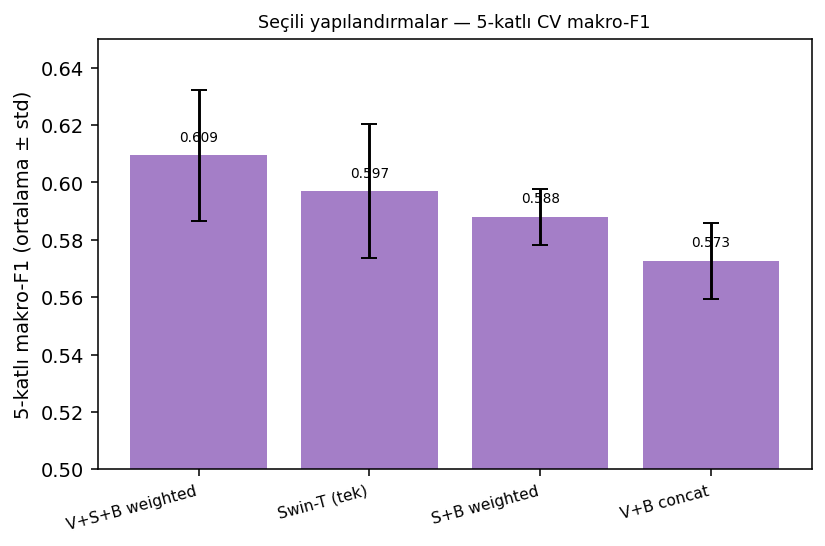
\includegraphics[width=0.6\linewidth]{cv_macrof1_bar.png}
  \caption{Seçili yapılandırmaların 5-katlı makro-F1 değerleri (ortalama $\pm$
  standart sapma). Üçlü ağırlıklı füzyon en yüksek ortalamaya sahiptir.}
  \label{fig:cvbar}
\end{figure}

\subsection{Nihai modelin ayrıntılı çözümlemesi}
Nihai modeli (fold 0) daha yakından inceliyoruz: önce eğitim dinamiği, ardından
havuzlanmış karışıklık matrisi ile sınıf bazında başarım ele alınır.

\subsubsection{Eğitim dinamiği}
Şekil~\ref{fig:curves} nihai modelin (0.~kat) eğitim eğrilerini gösterir; eğitim
kaybı düzenli azalırken doğrulama makro-F1'i erken bir epoch'ta tepe yapar ve
erken durdurma devreye girer.

\subsubsection{Karışıklık matrisi ve sınıf bazında başarım}
Şekil~\ref{fig:cm} havuzlanmış OOF karışıklık
matrisidir. Yaygın sınıflar çok yüksek köşegen değerlerine sahiptir
(ör.\ \texttt{normal-pylorus} $0{,}99$, \texttt{retroflex-stomach} $0{,}99$,
\texttt{impacted-stool} $0{,}99$), buna karşılık hataların büyük kısmı
\emph{anlamsal/anatomik olarak komşu} sınıflar arasında yoğunlaşır: ülseratif
kolit dereceleri birbirine karışır, \texttt{hemorroids} büyük ölçüde
\texttt{retroflex-rectum} olarak tahmin edilir ve \texttt{oesophagitis-a}
\texttt{normal-z-line} ile karışır.

\begin{figure}[H]
  \centering
  \begin{subfigure}{0.48\linewidth}
    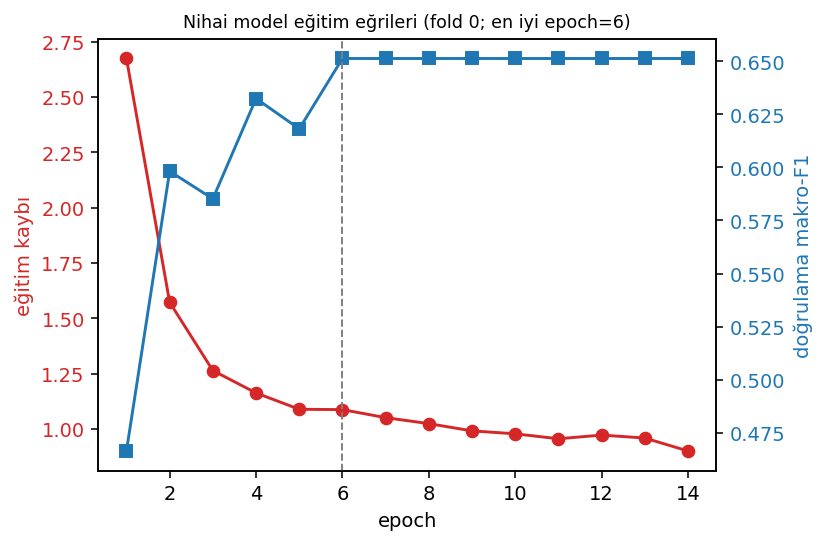
\includegraphics[width=\linewidth]{training_curves.png}
    \caption{Eğitim eğrileri (0.~kat).}
    \label{fig:curves}
  \end{subfigure}\hfill
  \begin{subfigure}{0.48\linewidth}
    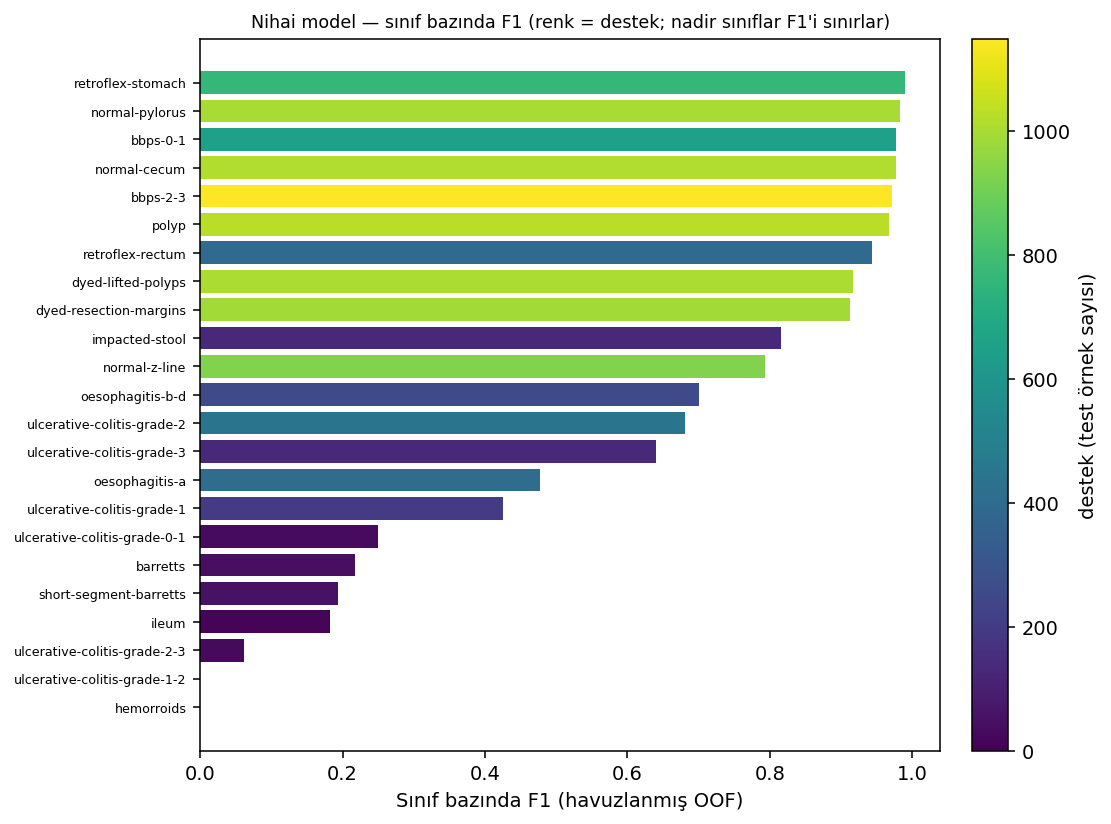
\includegraphics[width=\linewidth]{per_class_f1.png}
    \caption{Sınıf bazında F1 (renk = destek).}
    \label{fig:pcf1}
  \end{subfigure}
  \caption{Nihai modelin eğitim dinamikleri ve sınıf bazında başarımı. Düşük
  destekli sınıflar düşük F1 ile güçlü biçimde ilişkilidir.}
\end{figure}

\begin{figure}[H]
  \centering
  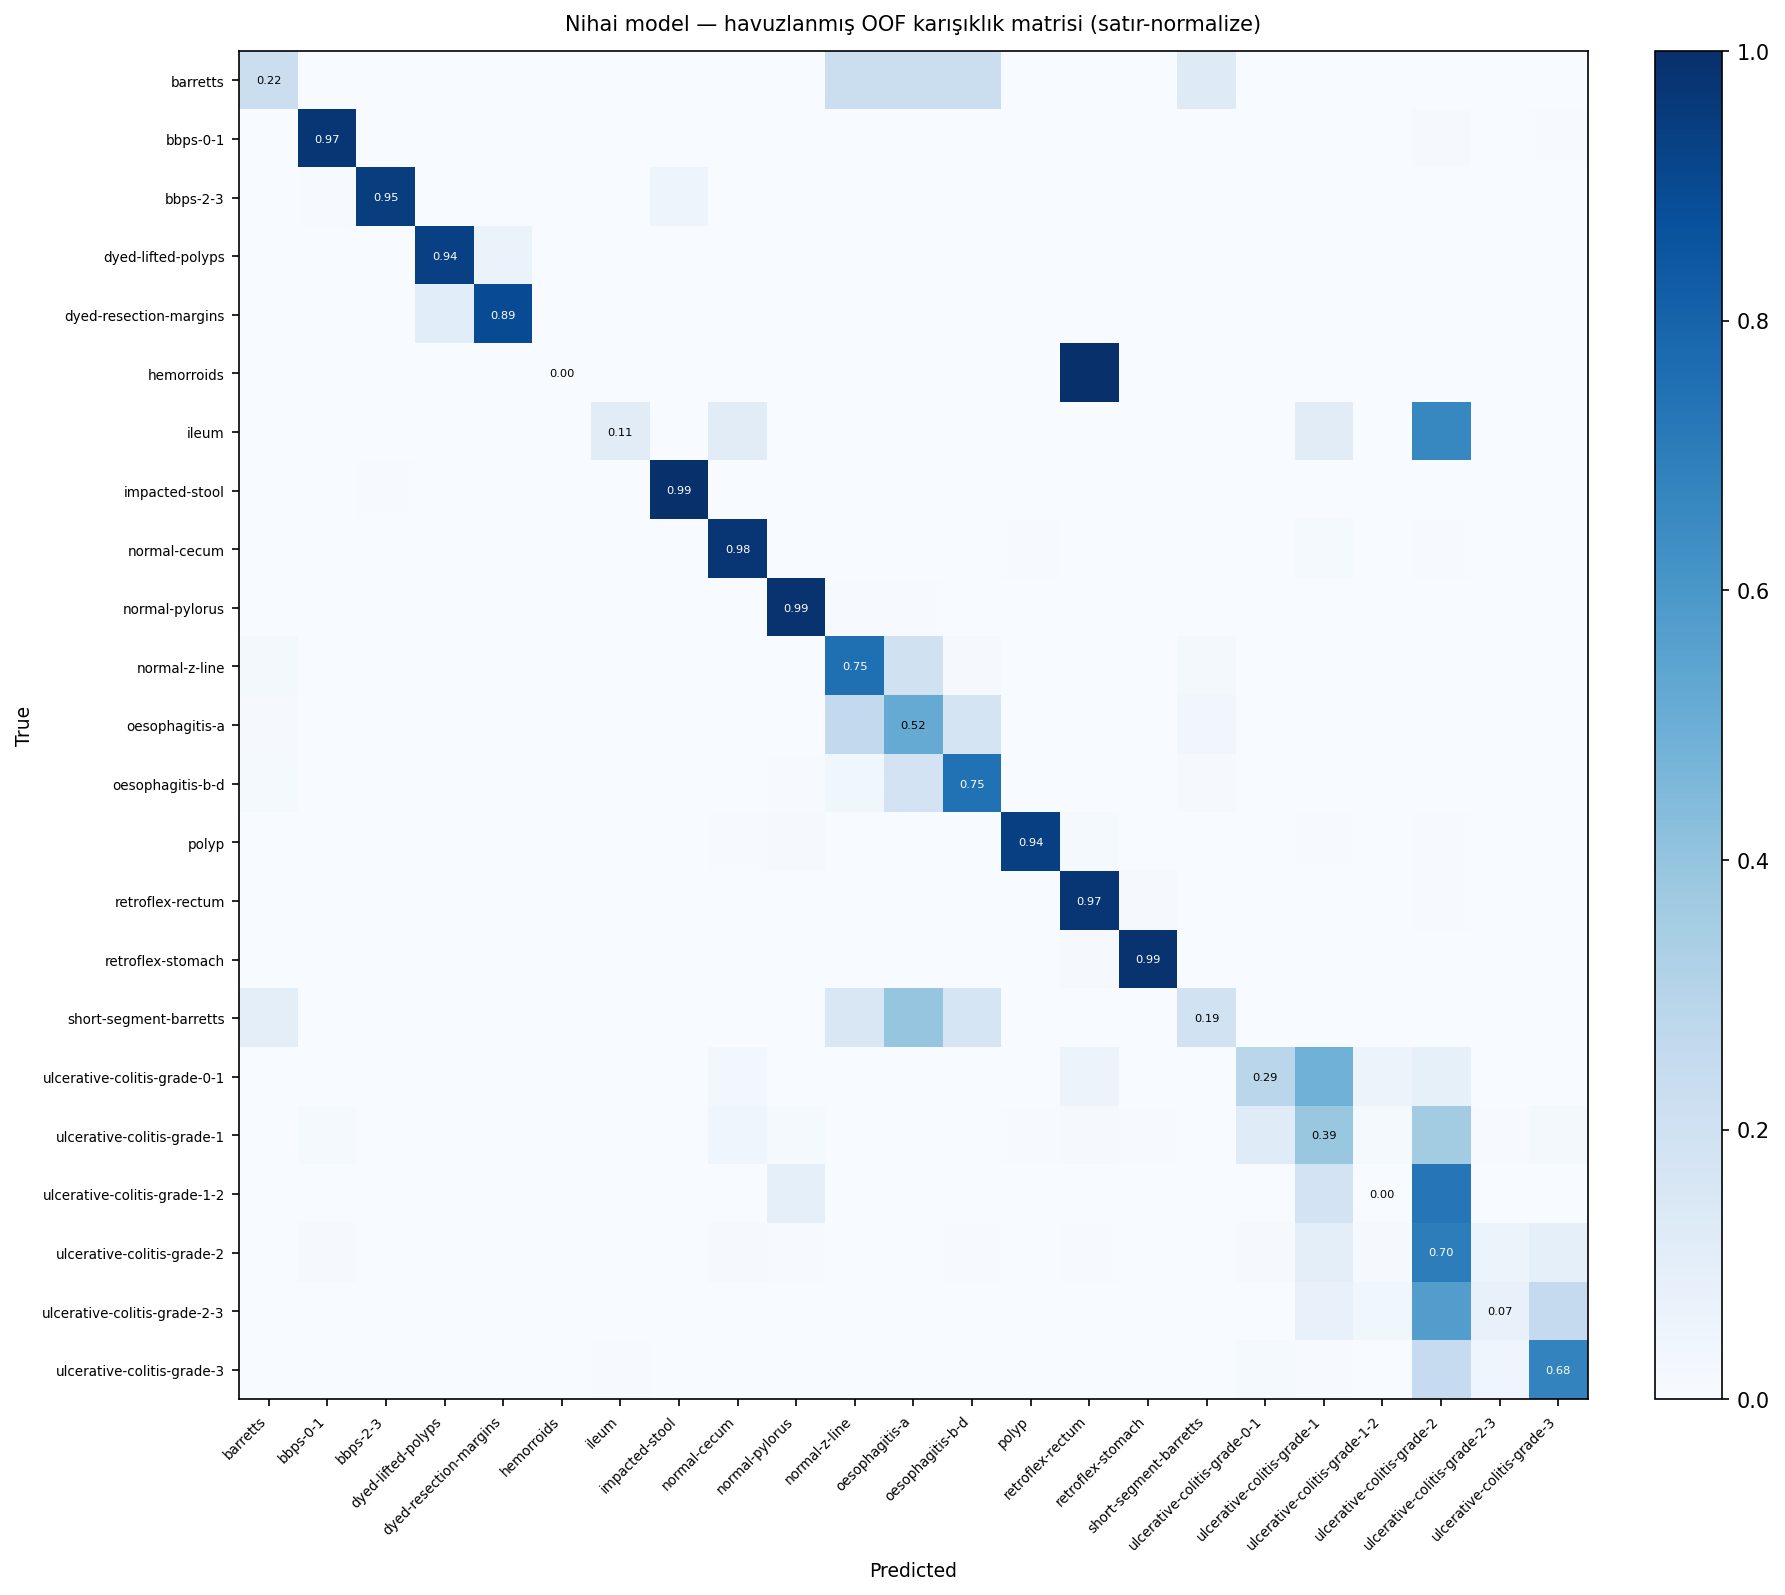
\includegraphics[width=0.92\linewidth]{confusion_matrix.png}
  \caption{Nihai modelin havuzlanmış ($n=10{.}662$) OOF karışıklık matrisi
  (satır-normalize). Hatalar büyük ölçüde anatomik/ordinal komşu sınıflar
  arasındadır.}
  \label{fig:cm}
\end{figure}

Sınıf bazında metrikler (Tablo~\ref{tab:perclass}) bu tabloyu nicelleştirir:
yüksek destekli sınıflarda F1 $\approx 0{,}97$--$0{,}99$ iken, en düşük destekli
sınıflarda (\texttt{hemorroids}: 6, \texttt{ulcerative-colitis-grade-1-2}: 11)
F1 sıfıra kadar düşer.

Havuzlanmış OOF üzerinde, ana ölçüt makro-F1'in ($0{,}612$) yanında destekleyici
toplu ölçütler de hesaplanmıştır: doğruluk $0{,}878$ (tek-etiketli çok-sınıfta
mikro-F1'e eşittir), ağırlıklı F1 $0{,}879$ ve Matthews korelasyon katsayısı
(MCC) $0{,}868$. Makro-F1 ile bu toplu ölçütler arasındaki belirgin açık,
dengesizliğin etkisini bir kez daha ortaya koyar; MCC ($0{,}868$), veri kümesi
makalesinin en iyi CNN temelinin ($0{,}899$) biraz altında olmakla birlikte aynı
bütünsel uyum bandındadır.

\begin{table}[H]
  \centering
  \caption{Nihai model: en düşük ve en yüksek F1'li altı sınıf (havuzlanmış OOF).}
  \label{tab:perclass}
  \begin{tabular}{lccc}
    \toprule
    Sınıf & Kesinlik & Duyarlılık & F1 (Destek) \\
    \midrule
    hemorroids                     & $0{,}00$ & $0{,}00$ & $0{,}00$ (6) \\
    ulcerative-colitis-grade-1-2   & $0{,}00$ & $0{,}00$ & $0{,}00$ (11) \\
    ulcerative-colitis-grade-2-3   & $0{,}05$ & $0{,}07$ & $0{,}06$ (28) \\
    \midrule
    bbps-0-1                       & $0{,}98$ & $0{,}97$ & $0{,}98$ (646) \\
    normal-pylorus                 & $0{,}98$ & $0{,}99$ & $0{,}98$ (999) \\
    retroflex-stomach              & $0{,}99$ & $0{,}99$ & $0{,}99$ (764) \\
    \bottomrule
  \end{tabular}
\end{table}

\subsection{Toplamsal teknikler ve istatistiksel anlamlılık}
\label{sec:addons}
Nihai model üzerinde denenen toplamsal, sızıntısız teknikler
Tablo~\ref{tab:addons}'da özetlenmiştir. Test zamanı veri artırma (TTA) ve
sızıntısız seed topluluğu makro-F1'i güven aralığı düzeyinde ayırt edilebilir
biçimde artırmamıştır. Son-işlem logit düzeltmesi~\cite{menon2020logitadjust}
ise makro-F1'i \emph{düşürmüştür} (Şekil~\ref{fig:logit}): düzeltme gücü $\tau$
arttıkça başarım tekdüze azalır. Bunun nedeni, modelin zaten dengeli örnekleyici
ile eğitilmiş olması ve örtük önselin yaklaşık tekdüze olmasıdır; eğitim önselini
çıkarmak \emph{ikinci kez} düzeltme yaparak nadir sınıflara aşırı kayma getirir.

Buna karşılık, eşli \textbf{McNemar} testi~\cite{dietterich1998mcnemar}
($n=10{.}662$), üçlü füzyonun en iyi tekli omurgadan ($\chi^2_{cc}=15{,}25$,
$p=9{,}2\times10^{-5}$) ve en iyi ikili füzyondan ($\chi^2_{cc}=25{,}25$,
$p=4{,}7\times10^{-7}$) \emph{anlamlı biçimde daha doğru} olduğunu göstermiştir.
Bu, doğruluk düzeyinde bir testtir; makro-F1 güven aralıklarının kısmen
örtüşmesiyle çelişmez, onu tamamlar: füzyon genel olarak anlamlı sayıda doğru
tahmin ekler, ancak makro-F1 kazancı nadir sınıflarca sınırlanır.

\begin{table}[H]
  \centering
  \caption{Nihai model üzerinde toplamsal teknikler (havuzlanmış OOF makro-F1).
  Hiçbiri nihai modeli değiştirmez; tümü sızıntısızdır.}
  \label{tab:addons}
  \footnotesize
  \begin{tabularx}{\linewidth}{@{}l c X@{}}
    \toprule
    Teknik & Havuz makro-F1 & Not \\
    \midrule
    Temel (nihai model)        & $0{,}6119$ & ana sonuç \\
    Seed topluluğu             & $0{,}6157\;[0{,}5994,\,0{,}6321]$ & küçük artış; GA örtüşüyor; final model değişmedi \\
    TTA                        & $0{,}6105\;[0{,}5920,\,0{,}6280]$ & kazanım yok; GA örtüşüyor \\
    Logit düzeltmesi ($\tau{=}1$) & $0{,}4911$ & düşürür (aşırı düzeltme) \\
    GMU füzyonu (üçlü, 0.~kat) & $0{,}5525$ & ağırlıklının altında \\
    \bottomrule
  \end{tabularx}
\end{table}

\begin{figure}[H]
  \centering
  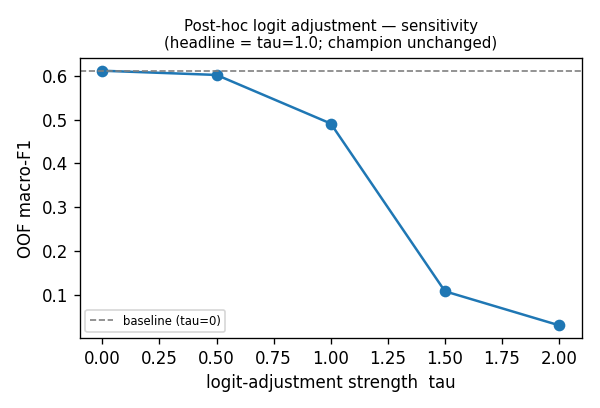
\includegraphics[width=0.5\linewidth]{logit_adjust_tau.png}
  \caption{Son-işlem logit düzeltmesi duyarlılık eğrisi: makro-F1, düzeltme gücü
  $\tau$ ile tekdüze azalır.}
  \label{fig:logit}
\end{figure}

\subsection{Literatürle bağlamsal karşılaştırma}
Sonuçları literatürle konumlandırırken iki noktayı ayrı ele alıyoruz: çalışmalar
arasındaki protokol/ölçüt farkları ve bu farkların metrik yorumuna etkisi.

\subsubsection{Protokol ve ölçüt farkları}
Literatürdeki HiperKvasir çalışmaları farklı bölme protokolleri ve farklı ölçüt
tanımları kullandığından, sayılar doğrudan değil \emph{bağlamsal} ele alınmalıdır.
Çalışmaların çoğu doğruluk veya genel/ağırlıklı F1 raporlar; sızıntıya karşı
denetlenmiş bir makro-F1 seyrek verilir. Veri kümesini tanıtan
çalışma~\cite{borgli2020hyperkvasir} bir istisnadır: iki-bölme ortalamasıyla
\emph{makro-ortalama} F1 raporladığından ölçüt türü bizimkiyle aynıdır, fakat bölme
protokolü farklıdır. GastroViT~\cite{gastrovit2025} bizimle aynı 23 sınıflı alt
kümeyi kullanır ancak topluluk ve farklı bölme ile çalışır; EffiMix~\cite{ramamurthy2022effimix}
ve HSW-ViT~\cite{wang2023hswvit} de farklı bölmelerde sonuç verir.

\begin{table}[H]
  \centering
  \footnotesize
  \caption{HiperKvasir bağlamsal konumlandırma (protokoller farklı; doğrudan kıyas
  değil). ``$-$'': karşılaştırılabilir makro-F1 bildirilmemiş. $^{\dagger}$Borgli'nin
  doğruluğu mikro-F1 olarak verilmiştir (tek-etiketli çok-sınıfta mikro-F1, doğruluğa
  eşittir).}
  \label{tab:context}
  \begin{tabularx}{\linewidth}{@{}l X l c c l@{}}
    \toprule
    Çalışma & Yöntem & Protokol & Doğ. & Makro-F1 & Diğer \\
    \midrule
    Bu çalışma & ViT füzyonu (V+S+B) & resmi 5-katlı + GA & $\approx$0,88 & \textbf{0,612} & MCC 0,868 \\
    Borgli 2020~\cite{borgli2020hyperkvasir} & CNN (DenseNet-161) & 2-bölme ort. & 0,907$^{\dagger}$ & 0,619 & MCC 0,899 \\
    GastroViT 2025~\cite{gastrovit2025} & ViT topluluğu & kendi bölmesi & 0,920 & $-$ & $-$ \\
    HSW-ViT 2023~\cite{wang2023hswvit} & HSW-ViT & kendi bölmesi & 0,868 & $-$ & $-$ \\
    EffiMix 2022~\cite{ramamurthy2022effimix} & karışım & kendi bölmesi & 0,980 & $-$ & ağ.\ F1 0,97 \\
    \bottomrule
  \end{tabularx}
\end{table}

\subsubsection{Metrik konumlandırma}
Makro-F1 ölçütünde sonucumuz ($0{,}612$), veri kümesi makalesinin CNN temel
sonuçlarının bandındadır (makro-F1 $0{,}605$–$0{,}619$); bu, üç ViT omurgasının
füzyonunun güçlü CNN temellerine yakın bir makro başarım sağladığını bağlamsal
olarak gösterir. Yüksek doğruluk değerleri (EffiMix $\approx$\%98, GastroViT
$\approx$\%92), farklı protokollerden ve dengesizlik altında iyimser olan
toplu/ağırlıklı ölçütlerden kaynaklanır; nitekim Borgli'de de makro-F1 ($\approx
0{,}62$) ile mikro-F1/doğruluk ($\approx 0{,}91$) arasındaki açık, bu raporda
gözlenen açıkla aynı dengesizlik olgusunu yansıtır. Bu nedenle güncel-en-iyi bir
başarı iddiasında bulunulmamış; konum bağlamsal olarak sunulmuştur.

\section{Tartışma}
\label{sec:discussion}

\subsection{Hangi omurga daha iyi öznitelik öğrendi?}
Dondurulmuş rejimde tek başına en güçlü omurga \textbf{Swin-T} olmuştur
(makro-F1 $0{,}576$); bu, hiyerarşik kaydırmalı-pencere yapısının yerel doku ve
çok ölçekli ipuçlarını (endoskopi görüntülerinde ayırt edici olan mukoza dokusu,
damarlanma ve lezyon sınırları) iyi yakaladığını düşündürür. Saf
ViT-B orta düzeyde, tek başına BEiT-B ise en zayıf omurgadır ($0{,}522$). Bu
sıralama, öznitelik uzayının UMAP görselleştirmesinde de görülür
(Şekil~\ref{fig:umapbranches}): ViT-B ve Swin-T izdüşümleri daha ayrık kümeler
oluştururken, BEiT-B dağılımı daha iç içedir. Bununla birlikte BEiT-B,
\emph{tamamlayıcı} bir sinyal taşıdığı için füzyonda yine de değerlidir; tek
başına zayıf olması, füzyondaki katkısını dışlamaz. Bu sıralama dondurulmuş eleme
tablosuyla (Tablo~\ref{tab:frozen}) tutarlıdır: Swin'in yerel-çok ölçekli önyargısı
endoskopinin doku ve sınır ipuçlarıyla uyumludur, ViT'in küresel öz-dikkati ve
BEiT'in öz-denetimli temsili ise farklı yönlerden katkı sağlayarak füzyonun en güçlü
tekil omurganın üzerine çıkmasını mümkün kılar.

\begin{figure}[H]
  \centering
  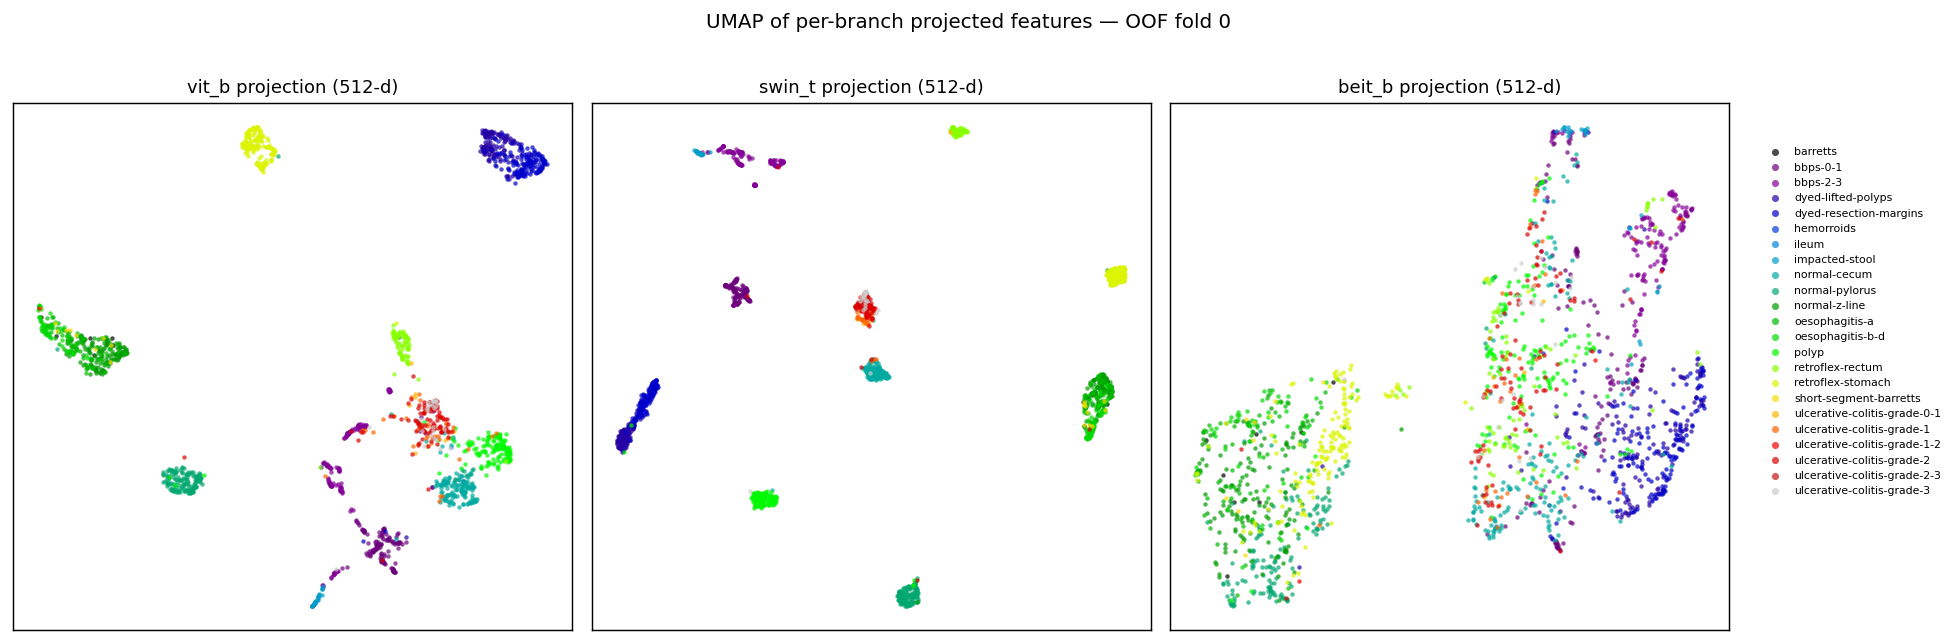
\includegraphics[width=0.95\linewidth]{umap_branches.png}
  \caption{Dal başına izdüşürülmüş 512 boyutlu özniteliklerin UMAP'i (OOF test).
  ViT-B ve Swin-T daha ayrık kümeler verir; BEiT-B daha dağınıktır.}
  \label{fig:umapbranches}
\end{figure}

\subsection{Füzyon işe yaradı mı?}
Evet, ancak sınırlı ölçüde. Üçlü ağırlıklı füzyon, en iyi tekli omurgaya kıyasla
hem ortalama hem havuzlanmış makro-F1'de önde olup
(Tablo~\ref{tab:cv}) eşli McNemar testinde \emph{istatistiksel olarak anlamlı}
biçimde daha doğrudur (Bölüm~\ref{sec:addons}). Yani çok-omurga füzyonu, genel
doğruluğa anlamlı bir katkı sağlar. Buna karşılık makro-F1 güven aralıkları
kısmen örtüşür; çünkü füzyonun eklediği doğru tahminler ağırlıklı olarak zaten
iyi sınıflandırılan yaygın sınıflardadır ve makro-F1, nadir sınıflarca
sınırlanır. \emph{Ağırlıklı} füzyon, \emph{birleştirmeden} daha iyi sonuç
vermiştir; bunun nedeni, birleştirmenin boyutu büyütüp daha fazla parametre
gerektirmesi ve küçük veri rejiminde aşırı uyuma daha açık olmasıdır. Gelişmiş
kapılı füzyon (GMU), özgün makaleye sadık öğe-bazında kapı uygulanmasına rağmen
ağırlıklı füzyonu geçememiştir (üçlü GMU $0{,}5525$); bu da daha karmaşık
füzyonun bu veri ölçeğinde ek kazanım getirmediğini gösterir.

\subsection{Hangi transfer yaklaşımı kazandı?}
Son blokların ince ayarı, her eleme adayında dondurulmuş rejimi geçmiştir
(Tablo~\ref{tab:transfer}). Bu beklenen bir sonuçtur: ImageNet ön-eğitimli
öznitelikler genel olsa da, son dönüştürücü bloklarının endoskopi alanına
uyarlanması ayırt ediciliği artırır. Süre açısından ince ayar, en iyi doğrulama
makro-F1'ine erken ulaşır (üçlü yapılandırmada 6.\ epoch; Tablo~\ref{tab:cost}),
dolayısıyla eğitim birkaç epoch içinde yakınsar. Dondurulmuş rejim daha hızlıdır
ve A100 gerektirmez; ince ayarın ek maliyeti ise verimlilik ayarlamalarıyla
(TF32, bfloat16, veri yükleyici paralelliği) yaklaşık $5$--$6\times$ azaltılarak
bütçe içinde tutulmuştur. Dengesizliği ele almak için \emph{ağırlıklı örnekleyici} doğru
mekanizma olmuştur; son-işlem logit düzeltmesinin başarımı düşürmesi
(Şekil~\ref{fig:logit}), örnekleyicinin dengesizliği zaten ele aldığını ve ek bir
önsel düzeltmesinin gereksiz/zararlı olduğunu doğrular.

\subsection{Yorumlanabilirlik: model neye bakıyor?}
Modelin karar gerekçelerini iki açıdan inceliyoruz: girdi üzerindeki dikkat ve
aktivasyon haritaları ile füzyon öznitelik uzayının yapısı.

\subsubsection{Dikkat ve Grad-CAM++}
Dikkat yayılımı ve Grad-CAM++ haritaları, doğru sınıflandırılan örneklerde
modelin \emph{klinik olarak anlamlı} bölgelere odaklandığını göstermektedir
(Şekil~\ref{fig:interp}). Örneğin retroflex konumundaki örneklerde model,
endoskobun retrofleksiyon bölgesine; pilor görüntülerinde ise pilor halkasına
yoğunlaşır. Hatalı örneklerde ise odak dağınıklaşır veya komşu yapıya kayar; bu,
karışıklık matrisindeki ordinal/anatomik karışmalarla tutarlıdır.

\begin{figure}[H]
  \centering
  \begin{subfigure}{0.48\linewidth}
    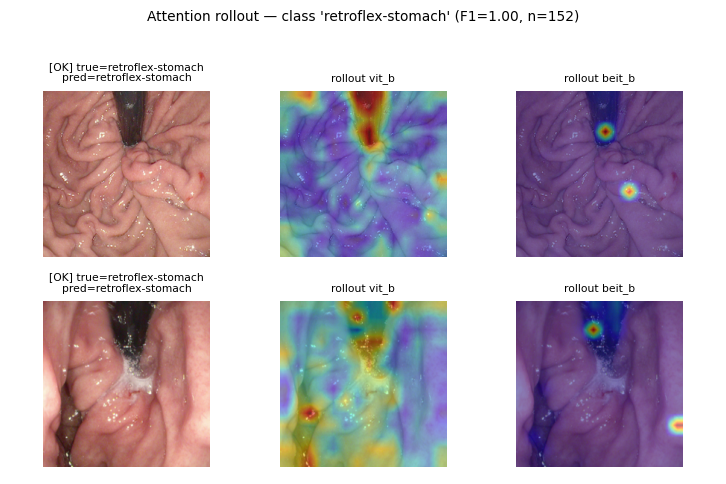
\includegraphics[width=\linewidth]{rollout_retroflex-stomach.png}
    \caption{Dikkat yayılımı (doğru sınıf).}
  \end{subfigure}\hfill
  \begin{subfigure}{0.48\linewidth}
    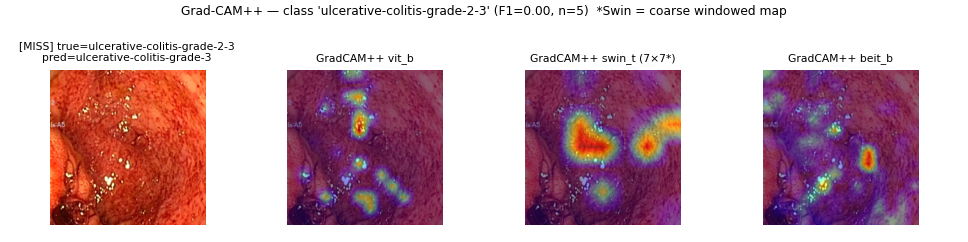
\includegraphics[width=\linewidth]{gradcam_ulcerative-colitis-grade-2-3.png}
    \caption{Grad-CAM++ (nadir sınıf, hata içeren panel).}
  \end{subfigure}
  \caption{Yorumlanabilirlik örnekleri. Doğru örneklerde odak klinik bölgededir;
  nadir/karışan sınıflarda odak dağılır. Swin dalının Grad-CAM++ haritası
  hiyerarşik pencere yerleşimi nedeniyle daha kaba ($7{\times}7$) olduğundan ilgili
  panelde dipnotla işaretlenmiştir.}
  \label{fig:interp}
\end{figure}

\subsubsection{Öznitelik uzayı (UMAP)}
Öznitelik uzayının füzyon sonrası UMAP'i (Şekil~\ref{fig:umapfused}), yaygın
sınıfların belirgin biçimde ayrıştığını, buna karşılık ülseratif kolit
derecelerinin iç içe geçtiğini gösterir; bu, makro-F1 tavanının doğrudan görsel
kanıtıdır.

\begin{figure}[H]
  \centering
  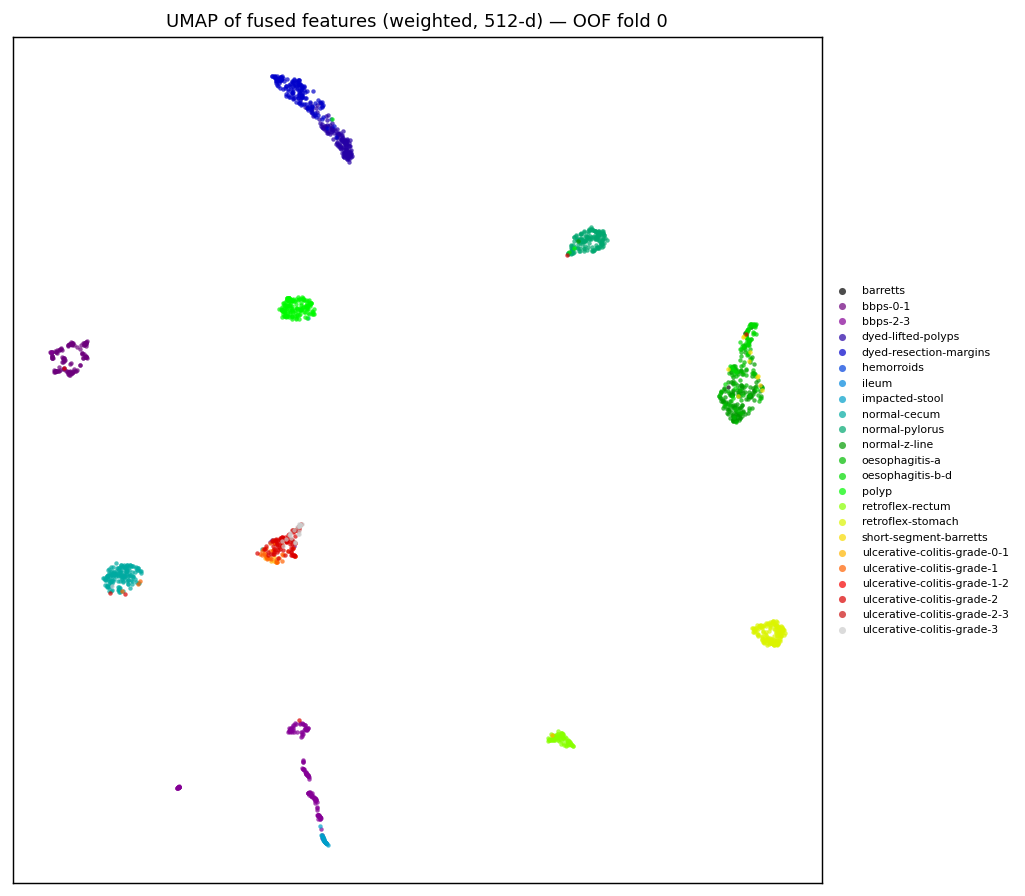
\includegraphics[width=0.6\linewidth]{umap_fused.png}
  \caption{Füzyon öznitelikleri UMAP'i (OOF test, 23 sınıf). Ayrık kümeler =
  kolay sınıflar; iç içe bölge = karışan nadir sınıflar (ör.\ kolit dereceleri).}
  \label{fig:umapfused}
\end{figure}

\subsection{Hata analizi ve sınıf karışmaları}
Karışıklık matrisi (Şekil~\ref{fig:cm}) ve sınıf bazında metrikler, hataların
rastgele dağılmadığını, büyük ölçüde \emph{anlamsal veya anatomik olarak komşu}
sınıflar arasında yoğunlaştığını gösterir. İlk hata türü \emph{ordinal} şiddet
karışmasıdır: ülseratif kolit dereceleri bitişik derecelere karışır; örneğin
grade-1-2 ve grade-2-3 gibi ara dereceler büyük ölçüde komşu tam dereceler olarak
tahmin edilir. Bu, derecelerin görsel olarak süreklilik göstermesi ve ara sınıfların
çok düşük destekli olmasının birleşik sonucudur. İkinci hata türü \emph{anatomik}
benzerliktir: \texttt{hemorroids} örnekleri ağırlıklı olarak \texttt{retroflex-rectum},
\texttt{oesophagitis-a} ise \texttt{normal-z-line} olarak sınıflandırılır; bu sınıf
çiftleri aynı anatomik bölgeyi paylaşır ve görünüm olarak yakındır. Buna karşılık
belirgin ve yüksek destekli sınıflar (\texttt{normal-pylorus},
\texttt{retroflex-stomach}, \texttt{impacted-stool}) köşegende neredeyse hatasızdır.
Klinik açıdan bu hatalar büyük ölçüde ``yakın'' hatalardır; tamamen ilgisiz sınıflara
kayma seyrektir.

\subsection{Dengesizliğin makro-F1 üzerindeki etkisi}
Makro-F1 her sınıfa eşit ağırlık verdiğinden, çok düşük destekli nadir sınıflardaki
düşük başarım, yüksek genel doğruluğa rağmen makro-F1'i belirgin biçimde aşağı çeker;
doğruluk (\%88) ile makro-F1 ($\approx 0{,}61$) arasındaki açık bunun doğrudan
ölçüsüdür. Bu davranış dengeli-hata bakış açısıyla tutarlıdır: dengesiz dağılımda
çoğunluk sınıfları toplu ölçütleri iyimser kılar~\cite{menon2020logitadjust}.
Dengesizliği ele almanın standart kaldıraçları arasında, iyi sınıflandırılan
örneklerin kaybını azaltıp zor ve nadir örneklere odaklanan odak kaybı
(focal loss)~\cite{lin2017focal} ve nadir sınıfları yeniden örnekleyen sınıf-dengeli
örnekleme bulunur. Bu çalışmada eğitimde ters-frekanslı ağırlıklı örnekleyici
kullanılmış, ayrıca son-işlem logit düzeltmesi denenmiştir. Logit düzeltmesinin
başarımı düşürmesi (Bölüm~\ref{sec:addons}), örnekleyicinin dengesizliği zaten ele
aldığını ve modelin örtük önselinin yaklaşık tekdüze olduğunu gösterir. Nadir
sınıflardaki temel sınır ise bir model değil veri kıtlığı sorunudur: bazı sınıfların
onlu sayılarda örneği vardır ve hiçbir kayıp ya da örnekleme düzenlemesi eksik veriyi
telafi edemez.

\subsection{Aynı protokol altında CNN füzyonu ile karşılaştırma}
\label{sec:cnnvit}
Aynı veri kümesi, aynı resmi 5-katlı protokol, sızıntıya karşı denetlenmiş OOF
değerlendirme ve aynı füzyon çerçevesi (birleştirme/ağırlıklı/GMU + MLP) altında
eğitilen CNN-omurgalı bir füzyon modeli, doğrudan ve kontrollü bir karşılaştırma
olanağı sağlar; yalnız omurga ailesi değişir (CNN: ResNet-50 + MobileNetV2 +
EfficientNet-B0). Tablo~\ref{tab:cnnvit} iki ailenin nihai modellerini karşılaştırır.

\begin{table}[H]
  \centering
  \caption{Kontrollü karşılaştırma: aynı veri kümesi, protokol ve füzyon çerçevesi
  altında CNN-omurgalı ve ViT-omurgalı füzyon (havuzlanmış OOF, $n=10{.}662$; makro-F1
  ana ölçüt). Reçete: ViT temel (TTA kazanç vermedi), CNN test zamanı veri artırmalı.}
  \label{tab:cnnvit}
  \begin{tabular}{llccc}
    \toprule
    Aile (omurgalar) & Reçete & Makro-F1 & Doğruluk & MCC \\
    \midrule
    ViT (ViT-B + Swin-T + BEiT-B) & temel & \textbf{0,6119} & 0,8779 & 0,868 \\
    CNN (ResNet-50 + MobileNetV2 + EfficientNet-B0) & +TTA & 0,6075 & 0,8765 & 0,866 \\
    \bottomrule
  \end{tabular}
\end{table}

İki aile istatistiksel olarak \emph{denktir}: makro-F1 güven aralıkları örtüşür,
doğruluk ve MCC değerleri neredeyse aynıdır. Aynı temel (TTA'sız) reçete altında bile
CNN füzyonunun makro-F1'i ($0{,}600$), ViT füzyonunun güven aralığı içinde kalır.
Dolayısıyla bir aile diğerine belirgin bir üstünlük sağlamaz; her ikisi de aynı
nadir-sınıf tavanına ulaşır. Bu bulgu, başarımı sınırlayan etkenin omurga ailesi
değil, düşük destekli sınıflardaki veri kıtlığı olduğunu güçlü biçimde destekler.

Bu ortak tavan, yöntemden bağımsız sonuçlarla da tutarlıdır: odak kaybı, test zamanı
veri artırma ve seed topluluğu gibi toplamsal teknikler her iki ailede de en iyi
çapraz-entropi yapılandırmasını güven aralığı düzeyinde geçememiştir. Yöntemsel olarak
bu çalışma, CNN-omurgalı füzyonun açık bıraktığı yönleri ele alır: dönüştürücü
omurgalar ile dikkat yayılımı ve Grad-CAM++ temelli yorumlanabilirlik burada
uygulanırken, iki ailede de kazanç sağlamayan teknikler bir kenara bırakılmıştır.

\subsection{Güçlü ve zayıf yönler}
Çalışmanın katkılarını ve sınırlarını, her birini mevcut bulgulara bağlayarak iki
başlık altında topluyoruz.

\subsubsection{Güçlü yönler}
\begin{itemize}
  \item \textbf{Anlamlı füzyon kazancı.} Üç tamamlayıcı ViT omurgasının ağırlıklı
        füzyonu, en iyi tekli omurgadan ve en iyi ikiliden eşli McNemar testinde
        istatistiksel olarak anlamlı biçimde daha doğrudur (Bölüm~\ref{sec:addons});
        ortalama ve havuzlanmış makro-F1'de de öndedir (Tablo~\ref{tab:cv}).
  \item \textbf{Temel-bandı makro başarım.} Makro-F1 ($0{,}612$) ve MCC ($0{,}868$),
        veri kümesi makalesinin CNN temellerinin bandındadır (Tablo~\ref{tab:context});
        bu, çok-ViT füzyonunun güçlü CNN temellerine yakın bir makro başarım sağladığını
        bağlamsal olarak gösterir.
  \item \textbf{Titiz değerlendirme.} Sızıntıya karşı denetlenmiş resmi 5-katlı
        protokol ve önyükleme \%95 güven aralıkları, sonuçların güvenilirliğini
        destekler (Tablo~\ref{tab:cv}).
  \item \textbf{Yorumlanabilirlik.} Dikkat yayılımı ve Grad-CAM++ haritaları
        kararların klinik bölgelerle ilişkili olduğunu, UMAP ise sınıf ayrışmasını
        gösterir (Şekil~\ref{fig:interp}, \ref{fig:umapfused}).
  \item \textbf{Dürüst ve eksiksiz analiz.} Kazanç sağlamayan teknikler (GMU, TTA,
        seed topluluğu, logit düzeltmesi) gizlenmeden raporlanmıştır
        (Tablo~\ref{tab:addons}, Şekil~\ref{fig:logit}).
  \item \textbf{Verimlilik.} İnce ayar maliyeti, verimlilik ayarıyla yaklaşık
        $5$--$6\times$ azaltılarak bütçe içinde tutulmuştur (Tablo~\ref{tab:cost}).
\end{itemize}

\subsubsection{Sınırlamalar}
\begin{itemize}
  \item \textbf{Nadir-sınıf tavanı.} Çok düşük destekli sınıflarda (ör.\
        \texttt{hemorroids}: 6, \texttt{ulcerative-colitis-grade-1-2}: 11) F1 sıfıra
        iner (Tablo~\ref{tab:perclass}); bu bir model değil \emph{veri kıtlığı}
        sınırıdır ve makro-F1'i belirleyen ana etkendir.
  \item \textbf{Sınırlı makro-F1 kazancı.} Füzyonun katkısı doğruluk düzeyinde
        anlamlı olsa da, makro-F1 güven aralıkları kısmen örtüşür; kazanç ağırlıklı
        olarak zaten iyi sınıflandırılan yaygın sınıflardan gelir.
  \item \textbf{Klinik olarak ``yakın'' hatalar.} Hatalar büyük ölçüde ordinal
        (kolit dereceleri) veya anatomik (\texttt{hemorroids}$\to$\texttt{retroflex-rectum})
        komşu sınıflar arasındadır.
  \item \textbf{Mimari sınırları.} Tek başına BEiT en zayıf omurgadır ve daha karmaşık
        kapılı füzyon (GMU) ağırlıklı füzyona ek kazanç getirmemiştir.
  \item \textbf{Yaklaşık üreme.} Ayarlı bfloat16/TF32 yolu, yalnızca çok düşük marjlı
        örneklerde nadir argmax değişimlerine yol açan yaklaşık bir üreme sağlar.
  \item \textbf{Tek veri kümesi.} Değerlendirme tek bir veri kümesi ve tek bölme
        protokolüyle sınırlıdır; klinik ya da dış doğrulama yapılmamıştır.
\end{itemize}

\section{Sonuç}
\label{sec:conclusion}

Bu çalışmada, HiperKvasir 23-sınıf GI endoskopi sınıflandırması için çoklu ViT
tabanlı bir özellik füzyonu yaklaşımı sunulmuştur. Üç tamamlayıcı omurganın
(ViT-B/16, Swin-T, BEiT-B/16) ağırlıklı füzyonunun ince ayarlı sürümü, resmi
5-katlı protokolde en iyi yapılandırma olmuş; havuzlanmış makro-F1
$0{,}6119$ (\%95 GA $[0{,}5930,\,0{,}6295]$), doğruluk $\approx 0{,}88$
elde edilmiştir. Bu yapılandırma, eşli McNemar testinde hem en iyi tekli
omurgadan hem de en iyi ikili füzyondan istatistiksel olarak anlamlı biçimde
daha doğrudur.

Çalışmanın temel çıkarımları şunlardır: (i)~çok-omurga füzyonu genel doğruluğa
anlamlı bir katkı sağlar, ancak makro-F1 kazancı nadir sınıflarca sınırlanır;
(ii)~ağırlıklı füzyon, birleştirme ve gelişmiş GMU füzyonundan daha iyi/eşdeğer
sonuç vermiştir; (iii)~son blokların ince ayarı dondurulmuş öznitelik çıkarımını
geçmiştir;
(iv)~dengesizlik için ağırlıklı örnekleyici yeterli olup son-işlem logit
düzeltmesi başarımı düşürmüştür. TTA ve seed topluluğu gibi toplamsal teknikler
güven aralığı düzeyinde ayırt edilebilir bir iyileşme getirmemiştir; bu, mimarinin
bu protokolde tavanına ulaştığını gösterir.

\paragraph{Sınırlamalar ve gelecek çalışmalar.} Temel sınırlama, çok düşük
destekli nadir sınıflardan kaynaklanan bir veri kıtlığıdır. Gelecekte;
(a)~ordinal yapıyı (ör.\ kolit dereceleri) açıkça modelleyen sıralı
sınıflandırma kayıpları, (b)~nadir sınıflar için hedefli veri toplama, üretici
artırma veya odak kaybı gibi dengesizlik-duyarlı kayıplar~\cite{lin2017focal}, ve
(c)~klinik açıdan ``yakın'' hataları ayrıştıracak ince taneli ayrım öğrenme
yaklaşımları umut verici yönlerdir. Bildirilen sayıların tümü
kaydedilen değerlendirme çıktılarına dayanır; literatür karşılaştırmaları
protokol farkları nedeniyle bağlamsaldır ve güncel-en-iyi bir başarı iddiasında
bulunulmamıştır.

\paragraph{Proje deposu.} Kaynak kod, eğitim çıktıları ve tanıtım videosu
bağlantısı proje deposunda yer alır:
\url{https://github.com/YasinEkici/hyperkvasir-multi-backbone-fusion}.


\appendix
\section{Sınıf bazında ayrıntılı metrikler}
\label{app:perclass}

Tablo~\ref{tab:perclass-full}, nihai modelin havuzlanmış OOF test kümesindeki
($n = 10{.}662$) 23 sınıfın tamamı için kesinlik, duyarlılık, F1 ve destek
değerlerini verir (F1'e göre artan sırada). Düşük destekli sınıflarla düşük F1
arasındaki güçlü ilişki açıkça görülür.

\begin{table}[H]
  \centering
  \footnotesize
  \caption{Nihai model: tüm sınıflar için sınıf bazında metrikler (havuzlanmış OOF).}
  \label{tab:perclass-full}
  \begin{tabular}{lcccr}
    \toprule
    Sınıf & Kesinlik & Duyarlılık & F1 & Destek \\
    \midrule
    hemorroids                     & $0{,}000$ & $0{,}000$ & $0{,}000$ & 6 \\
    ulcerative-colitis-grade-1-2   & $0{,}000$ & $0{,}000$ & $0{,}000$ & 11 \\
    ulcerative-colitis-grade-2-3   & $0{,}054$ & $0{,}071$ & $0{,}062$ & 28 \\
    ileum                          & $0{,}500$ & $0{,}111$ & $0{,}182$ & 9 \\
    short-segment-barretts         & $0{,}200$ & $0{,}189$ & $0{,}194$ & 53 \\
    barretts                       & $0{,}214$ & $0{,}220$ & $0{,}217$ & 41 \\
    ulcerative-colitis-grade-0-1   & $0{,}222$ & $0{,}286$ & $0{,}250$ & 35 \\
    ulcerative-colitis-grade-1     & $0{,}470$ & $0{,}388$ & $0{,}425$ & 201 \\
    oesophagitis-a                 & $0{,}442$ & $0{,}519$ & $0{,}477$ & 403 \\
    ulcerative-colitis-grade-3     & $0{,}608$ & $0{,}677$ & $0{,}641$ & 133 \\
    ulcerative-colitis-grade-2     & $0{,}664$ & $0{,}700$ & $0{,}681$ & 443 \\
    oesophagitis-b-d               & $0{,}660$ & $0{,}746$ & $0{,}700$ & 260 \\
    normal-z-line                  & $0{,}837$ & $0{,}754$ & $0{,}794$ & 932 \\
    impacted-stool                 & $0{,}692$ & $0{,}992$ & $0{,}815$ & 131 \\
    dyed-resection-margins         & $0{,}932$ & $0{,}894$ & $0{,}912$ & 989 \\
    dyed-lifted-polyps             & $0{,}896$ & $0{,}937$ & $0{,}916$ & 1002 \\
    retroflex-rectum               & $0{,}914$ & $0{,}974$ & $0{,}943$ & 391 \\
    polyp                          & $0{,}995$ & $0{,}941$ & $0{,}967$ & 1028 \\
    bbps-2-3                       & $0{,}996$ & $0{,}948$ & $0{,}971$ & 1148 \\
    bbps-0-1                       & $0{,}980$ & $0{,}974$ & $0{,}977$ & 646 \\
    normal-cecum                   & $0{,}977$ & $0{,}976$ & $0{,}977$ & 1009 \\
    normal-pylorus                 & $0{,}978$ & $0{,}987$ & $0{,}983$ & 999 \\
    retroflex-stomach              & $0{,}991$ & $0{,}988$ & $0{,}990$ & 764 \\
    \bottomrule
  \end{tabular}
\end{table}

\section{Ek yorumlanabilirlik panelleri}
\label{app:interp}

Şekil~\ref{fig:interp-extra}, ana metni tamamlayan ek örnekler sunar: yaygın ve
iyi sınıflandırılan bir sınıfta dikkat yayılımı ile çok düşük destekli, hatalı
sınıflandırılan bir sınıfta Grad-CAM++. Yaygın sınıfta odak klinik bölgede
toplanırken, nadir sınıfta dağınıklaşır.

\begin{figure}[H]
  \centering
  \begin{subfigure}{0.9\linewidth}
    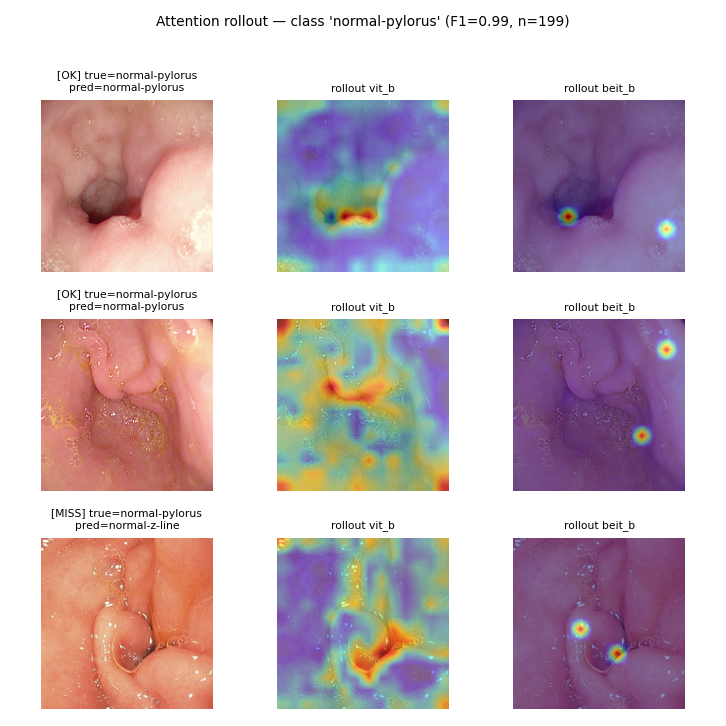
\includegraphics[width=\linewidth]{rollout_normal-pylorus.png}
    \caption{Dikkat yayılımı: \texttt{normal-pylorus} (yaygın, doğru).}
  \end{subfigure}\\[0.6em]
  \begin{subfigure}{0.9\linewidth}
    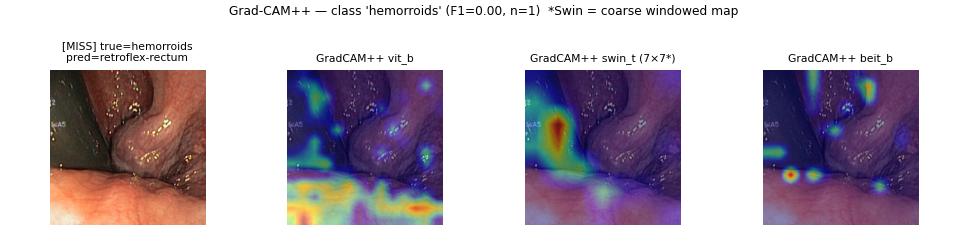
\includegraphics[width=\linewidth]{gradcam_hemorroids.png}
    \caption{Grad-CAM++: \texttt{hemorroids} (çok düşük destek, hata).}
  \end{subfigure}
  \caption{Ek yorumlanabilirlik panelleri. Üst: yaygın bir sınıfta dikkat
  yayılımı; alt: nadir bir sınıfta Grad-CAM++ (Swin dalı hiyerarşik pencere
  yerleşimi nedeniyle daha kaba bir harita verir).}
  \label{fig:interp-extra}
\end{figure}


\bibliographystyle{plain}
\bibliography{references}

\end{document}
